\documentclass[12pt]{report}

\usepackage[language=english, type=bachelor]{style}
\usepackage{enumitem}
\usepackage{indentfirst}
\usepackage{listings}
\usepackage{xcolor}
\usepackage{float}
\usepackage{tabularx}
\usepackage{booktabs}
\usepackage{caption}
\usepackage{subcaption}

% Python code highlighting
\definecolor{codegreen}{rgb}{0,0.6,0}
\definecolor{codegray}{rgb}{0.5,0.5,0.5}
\definecolor{codepurple}{rgb}{0.58,0,0.82}
\definecolor{backcolour}{rgb}{0.97,0.97,0.95}
\definecolor{codeblue}{rgb}{0.13,0.13,0.80}

\lstdefinestyle{pythonstyle}{
    backgroundcolor=\color{backcolour},
    commentstyle=\color{codegreen},
    keywordstyle=\color{codeblue}\bfseries,
    numberstyle=\tiny\color{codegray},
    stringstyle=\color{codepurple},
    basicstyle=\ttfamily\footnotesize,
    breakatwhitespace=false,
    breaklines=true,
    captionpos=b,
    keepspaces=true,
    numbers=left,
    numbersep=5pt,
    showspaces=false,
    showstringspaces=false,
    showtabs=false,
    tabsize=4,
    frame=single,
    framerule=0.4pt,
    rulecolor=\color{codegray},
}

\lstset{style=pythonstyle}

\lstdefinelanguage{yaml}{
    keywords={true,false,null,y,n},
    sensitive=false,
    comment=[l]{\#},
    morestring=[b]',
    morestring=[b]",
}

\usepackage{amsmath}
\usepackage{fancyhdr}
\pagestyle{fancy}
\lhead{}
\chead{}
\setlength{\headheight}{14.5pt}
\addtolength{\topmargin}{-2.5pt}
\renewcommand{\headrulewidth}{0.2pt}
\renewcommand{\footrulewidth}{0.2pt}

\begin{document}

% English title page
\specialization{\\ Business Information Systems}
\title{Reddit Sentiment Explorer: A Query-Driven Web Platform \\ for Analyzing Public Opinion Using Large Language Models}
\author{Dániel AIERIZER}
\supervisor{Associate Prof. Dénes CSALA, PhD}
\maketitle

% Romanian title page
\setbool{@eng}{false}
\specialization{\\Informatica Economică}
\title{Reddit Sentiment Explorer: O Platformă Web Bazată pe Interogări pentru Analiza Opiniei Publice Folosind Modele Lingvistice de Mari Dimensiuni}
\author{Dániel AIERIZER}
\supervisor{Lect. univ. dr. Dénes CSALA}
\maketitle

% Hungarian title page
\setbool{@hun}{true}
\specialization{\\ Gazdaság Informatika}
\title{Reddit Sentiment Explorer: Lekérdezés-alapú Webes Platform Közvélemény Elemzésére Nagy Nyelvi Modellek Segítségével}
\author{Dániel AIERIZER}
\supervisor{Dr. Dénes CSALA egyetemi adjunktus}
\maketitle

% Reset to English
\setbool{@eng}{true}
\setbool{@hun}{false}

\newpage
\pagenumbering{roman}

\begin{center}
  {\fontsize{14}{18} \textbf{Abstract}}
\end{center}

Social media platforms contain vast amounts of public opinion data, yet extracting structured sentiment insights from them remains a challenge. In this thesis, I present Reddit Sentiment Explorer, a query-driven web platform that enables users to analyze sentiment across Reddit communities for arbitrary search terms. The system collects posts and comments from Reddit via the Arctic Shift archive, filters them by language, matches them against user-supplied search terms, and classifies each matched document using a large language model through the OpenAI API. Classification results use a five-point sentiment scale ranging from very negative to very positive, accompanied by confidence scores, rationale, and evidence phrases extracted from the source text. The platform aggregates these results into interactive visualizations including sentiment timelines, distribution charts, subreddit breakdowns, and heatmaps, all presented through a Plotly Dash dashboard. The backend is built with FastAPI and SQLAlchemy on PostgreSQL, with an asynchronous worker that processes query runs independently. The entire system is containerized with Docker Compose for straightforward deployment. I evaluate the platform through a system demonstration and discuss the strengths and limitations of using large language models for sentiment classification of informal, multilingual social media text. The result is a modular, extensible tool that bridges the gap between ad-hoc sentiment analysis scripts and commercial social listening platforms.

\vspace{1em}

\textbf{Keywords:} sentiment analysis, Reddit, large language models, natural language processing, web application, Python, FastAPI, Plotly Dash

\vspace{2em}

\begin{center}
  {\fontsize{14}{16} \textbf{Összefoglaló}}
\end{center}

\begin{sloppypar}
A közösségi média platformok hatalmas mennyiségű közvélemény-adatot tartalmaznak, de a strukturált érzelemfelismerési betekintések kinyerése továbbra is kihívást jelent. Ebben a dolgozatban bemutatom a Reddit Sentiment Explorer-t, egy lekérdezés-alapú webes platformot, amely lehetővé teszi a felhasználók számára, hogy tetszőleges keresési kifejezések alapján elemezzék az érzelmi tónust a Reddit közösségeken keresztül. A rendszer az Arctic Shift archívumon keresztül gyűjti a bejegyzéseket és hozzászólásokat, nyelv szerint szűri azokat, egyezteti a felhasználó által megadott keresési kifejezésekkel, majd minden egyeztetett dokumentumot egy nagy nyelvi modell segítségével osztályoz az OpenAI API-n keresztül. Az osztályozás egy ötfokú érzelmi skálát használ, amelyhez konfidencia-pontszámok, indoklás és a forrásszövegből kiemelt bizonyíték-kifejezések tartoznak. A platform interaktív vizualizációkba összesíti az eredményeket, beleértve az érzelmi idővonalakat, eloszlási diagramokat, subreddit-bontásokat és hőtérképeket, amelyeket egy Plotly Dash vezérlőpulton mutat be. Az eredmény egy moduláris, bővíthető eszköz, amely áthidalja a szakadékot az ad-hoc érzelemelemzési szkriptek és a kereskedelmi közösségi figyelő platformok között.
\end{sloppypar}

\vspace{2em}

\begin{center}
  {\fontsize{14}{16} \textbf{Rezumat}}
\end{center}

Platformele de social media conțin cantități vaste de date privind opinia publică, însă extragerea de informații structurate despre sentimente rămâne o provocare. În această lucrare, prezint Reddit Sentiment Explorer, o platformă web bazată pe interogări care permite utilizatorilor să analizeze sentimentele din comunitățile Reddit pentru termeni de căutare arbitrari. Sistemul colectează postări și comentarii de pe Reddit prin arhiva Arctic Shift, le filtrează după limbă, le potrivește cu termenii de căutare furnizați de utilizator și clasifică fiecare document folosind un model lingvistic de mari dimensiuni prin API-ul OpenAI. Clasificarea utilizează o scală de sentiment în cinci puncte, însoțită de scoruri de încredere, raționament și expresii de evidență extrase din textul sursă. Platforma agregă aceste rezultate în vizualizări interactive, inclusiv cronologii ale sentimentelor, diagrame de distribuție, defalcări pe subreddit-uri și hărți de căldură, toate prezentate printr-un tablou de bord Plotly Dash. Rezultatul este un instrument modular și extensibil care acoperă distanța dintre scripturile ad-hoc de analiză a sentimentelor și platformele comerciale de monitorizare a rețelelor sociale.


\tableofcontents
\newpage

\fontsize{14}{18} \textbf{Abbreviations}
\begin{description}[align=left, labelwidth=2cm, leftmargin=!, itemsep=1.5pt]
  \item[API] Application Programming Interface
  \item[CRUD] Create, Read, Update, Delete
  \item[CSS] Cascading Style Sheets
  \item[ETL] Extract, Transform, Load
  \item[HTML] HyperText Markup Language
  \item[HTTP] Hypertext Transfer Protocol
  \item[JSON] JavaScript Object Notation
  \item[LLM] Large Language Model
  \item[NLP] Natural Language Processing
  \item[ORM] Object-Relational Mapping
  \item[REST] Representational State Transfer
  \item[SQL] Structured Query Language
  \item[TTL] Time to Live
  \item[UI] User Interface
  \item[URL] Uniform Resource Locator
  \item[UUID] Universally Unique Identifier
  \item[UX] User Experience
\end{description}

\newpage
\pagenumbering{arabic}

\chapter{Introduction}
\label{ch:introduction}

Every day, millions of users share opinions on Reddit across more than 100,000 active communities. These communities, called subreddits, cover virtually every topic imaginable, from technology and finance to food and local culture. For researchers, marketers, and curious individuals, this represents an enormous source of public opinion data. However, extracting structured sentiment insights from Reddit is far from straightforward. The text is informal, multilingual, rich in sarcasm, and spread across thousands of threads. Manual reading does not scale, and existing tools are either narrowly scoped academic scripts or expensive commercial platforms with rigid interfaces.

In this thesis, I present Reddit Sentiment Explorer, a query-driven web platform that allows any user to type a search term, select target subreddits and a content language, and receive a comprehensive sentiment analysis complete with interactive charts, timelines, and access to the original matched documents. The system leverages a large language model to classify each matched piece of content on a five-point sentiment scale, producing not just a label but also a confidence score, a rationale, and evidence phrases quoted directly from the source text.

\section{Motivation and Background}
\label{sec:motivation}

Sentiment analysis is one of the most widely studied tasks in natural language processing. Organizations use it to understand customer feedback, track brand perception, and monitor public discourse around events or policies \cite{liu2012sentiment}. Social media platforms are particularly attractive targets because they capture unfiltered, real-time public opinion from diverse populations.

Reddit stands out among social media platforms for several reasons. First, its community-based structure means that discussions are organized by topic, making it possible to target specific interest groups. Second, Reddit users tend to write longer, more detailed posts compared to platforms like Twitter, which historically imposed a 280-character limit. Third, Reddit data has been extensively used in academic research, with the Pushshift archive providing historical access to billions of posts and comments \cite{baumgartner2020pushshift}.

Despite these advantages, performing sentiment analysis on Reddit remains a manual, fragmented process for most practitioners. A researcher interested in how people feel about a specific product, policy, or cultural phenomenon must write custom scraping code, apply a classification model, and build their own visualizations. There is no widely available, open-source tool that combines all of these steps into a single, interactive experience. This gap is what Reddit Sentiment Explorer addresses.

The emergence of large language models such as GPT-4 has opened new possibilities for text classification \cite{brown2020language}. Unlike traditional machine learning models that require labeled training data for each specific task, large language models can classify text in a zero-shot or few-shot manner through prompt engineering. This makes them particularly suitable for a general-purpose sentiment analysis tool where the search terms and topics change with every query.

\section{Research Questions}
\label{sec:research_questions}

This thesis addresses two research questions:

\begin{enumerate}
    \item \textbf{How can a modular, query-driven system be designed to collect, filter, and classify Reddit content by sentiment for arbitrary user-defined search terms?}

    This question concerns the system architecture and pipeline design. It asks how the various concerns of data collection, text matching, language filtering, sentiment classification, and result aggregation can be separated into distinct, maintainable components while still producing a cohesive user experience.

    \item \textbf{How effectively can large language models classify sentiment in informal, multilingual social media text compared to simpler heuristic approaches?}

    This question concerns the quality of the sentiment classification. It asks whether prompting a large language model produces meaningful, interpretable results on the kind of text found on Reddit, and how these results compare to a baseline heuristic provider.
\end{enumerate}

\section{Methodology}
\label{sec:methodology}

I follow a software engineering methodology that consists of four phases:

\begin{enumerate}
    \item \textbf{Requirements analysis.} I identify the functional and non-functional requirements for the platform based on the use case of ad-hoc sentiment exploration of Reddit content.

    \item \textbf{Architecture design.} I design a four-service architecture consisting of a REST API, an asynchronous background worker, an interactive dashboard, and a PostgreSQL database. I define the data model, the query pipeline, and the sentiment provider abstraction.

    \item \textbf{Implementation.} I implement the system in Python using FastAPI for the API, Plotly Dash for the dashboard, SQLAlchemy for database access, and the OpenAI API for sentiment classification. The system is containerized with Docker Compose.

    \item \textbf{Evaluation.} I evaluate the system through a complete demonstration walkthrough and a discussion of the sentiment classification quality, comparing the large language model provider against a heuristic mock provider.
\end{enumerate}

\section{Thesis Structure}
\label{sec:thesis_structure}

The remainder of this thesis is organized as follows:

\textbf{Chapter~\ref{ch:literature_review}} reviews the relevant literature across four themes: sentiment analysis techniques, Reddit as a data source, large language models for text classification, and web application architectures for data-intensive systems.

\textbf{Chapter~\ref{ch:system_design}} presents the system design, including the requirements analysis, the high-level architecture, the data model, the query pipeline, and the sentiment classification strategy.

\textbf{Chapter~\ref{ch:implementation}} describes the implementation in detail, covering the technology stack, data collection, text matching, sentiment classification, aggregation, the API and worker, the interactive dashboard, and the deployment setup.

\textbf{Chapter~\ref{ch:results}} demonstrates the system through a walkthrough of a complete query lifecycle and discusses the sentiment classification quality and system performance.

\textbf{Chapter~\ref{ch:conclusions}} summarizes the contributions, discusses limitations, and outlines directions for future work.

\chapter{Literature Review}
\label{ch:literature_review}

This chapter reviews the academic and technical literature that provides the foundation for Reddit Sentiment Explorer. I organize the review around four themes: sentiment analysis as a field, Reddit as a data source for opinion mining, large language models for text classification, and web application architectures for data-intensive systems. The chapter concludes with a synthesis of the identified gaps that motivate the design decisions in subsequent chapters.

\section{Sentiment Analysis}
\label{sec:sentiment_analysis}

Sentiment analysis, also referred to as opinion mining, is the computational study of people's opinions, sentiments, and emotions expressed in text \cite{liu2012sentiment}. The field has grown significantly since the early work of \citeA{pang2002thumbs}, who demonstrated that machine learning classifiers could determine whether movie reviews were positive or negative with accuracy exceeding 80\%.

\subsection{Approaches to Sentiment Analysis}

Three broad approaches dominate the sentiment analysis literature: lexicon-based, machine learning, and deep learning methods.

\textbf{Lexicon-based methods} rely on dictionaries of words annotated with sentiment polarity. VADER (Valence Aware Dictionary and sEntiment Reasoner) is one of the most widely used lexicon-based tools, specifically designed for social media text \cite{hutto2014vader}. VADER uses a combination of a sentiment lexicon and grammatical rules to handle features common in social media, such as capitalization for emphasis and emoticons. While lexicon-based methods are fast and require no training data, they struggle with context-dependent sentiment, sarcasm, and domain-specific vocabulary.

\textbf{Machine learning methods} train classifiers on labeled datasets. \citeA{pang2002thumbs} compared Naive Bayes, maximum entropy, and support vector machine classifiers on movie review data. Support vector machines achieved the best performance in their experiments. Later work by \citeA{go2009twitter} applied similar techniques to Twitter data, using emoticons as distant supervision labels to create a large training set without manual annotation. The main limitation of traditional machine learning approaches is their dependence on feature engineering and domain-specific training data.

\textbf{Deep learning methods} use neural network architectures that learn feature representations directly from text. \citeA{kim2014convolutional} showed that convolutional neural networks applied to pre-trained word embeddings achieve strong results on sentence-level sentiment classification. \citeA{devlin2019bert} introduced BERT (Bidirectional Encoder Representations from Transformers), a pre-trained language model that can be fine-tuned for sentiment analysis with relatively small labeled datasets. BERT and its variants set new state-of-the-art benchmarks across multiple sentiment analysis datasets.

\subsection{Fine-Grained Sentiment Classification}

Most early sentiment analysis work focused on binary classification (positive vs. negative). However, many applications require finer granularity. \citeA{socher2013recursive} introduced the Stanford Sentiment Treebank, which provides sentiment labels at five levels: very negative, negative, neutral, positive, and very positive. This five-class formulation captures the intensity of sentiment, not just its polarity.

Fine-grained classification is more challenging than binary classification. \citeA{socher2013recursive} reported that their Recursive Neural Tensor Network achieved 45.7\% accuracy on five-class classification compared to 85.4\% on binary classification. The difficulty arises from the subtlety of distinguishing between adjacent classes such as ``negative'' and ``very negative,'' which often depends on nuanced contextual cues.

Reddit Sentiment Explorer adopts the five-class sentiment scale because it provides richer information for exploratory analysis. Users can see not just whether a community is positive or negative about a topic, but how strongly those sentiments are expressed.

\subsection{Challenges with Social Media Text}

Social media text presents several challenges for sentiment analysis. \citeA{rosenthal2017semeval} summarized these challenges in the context of the SemEval shared tasks on sentiment analysis in Twitter: informal language, abbreviations, misspellings, sarcasm, mixed sentiments within a single post, and the use of hashtags and mentions as sentiment signals.

\citeA{maynard2014challenges} specifically addressed the challenge of sarcasm detection, noting that sarcastic statements often express the opposite of their literal meaning. This is particularly relevant for Reddit, where sarcasm is a prevalent communication style in many communities.

\section{Reddit as a Data Source}
\label{sec:reddit_data_source}

Reddit is a social news aggregation and discussion platform founded in 2005. As of 2024, it has over 50 million daily active users across more than 100,000 active communities \cite{reddit2024statistics}. Its structure of subreddits, posts (also called submissions), and nested comment threads makes it a rich source for opinion mining.

\subsection{Structure and Content}

Each subreddit functions as a self-moderated community focused on a specific topic. Posts can contain text, links, images, or videos, and each post generates a tree of nested comments. Both posts and comments receive upvotes and downvotes from community members, producing a score that reflects community reception. This voting mechanism provides an additional signal beyond the text content itself.

Reddit content varies substantially across subreddits. Technical subreddits like r/programming tend to have formal, detailed discussions, while humor-oriented subreddits may contain mostly short, colloquial text. This diversity means that any analysis tool must handle a wide range of writing styles and levels of formality.

\subsection{Data Access}

Reddit's official API provides programmatic access to current content but imposes rate limits and does not provide historical data efficiently. To address this, \citeA{baumgartner2020pushshift} created the Pushshift archive, which provides bulk access to historical Reddit data going back to 2005. Pushshift has been widely used in academic research, with the dataset being cited in hundreds of studies.

Following changes to Reddit's API policies in 2023, Pushshift access was restricted. The Arctic Shift project emerged as a community-maintained alternative, providing similar historical archive access through a publicly available API. Reddit Sentiment Explorer uses Arctic Shift as its data source, which provides access to both historical and recent posts and comments with flexible search parameters.

\subsection{Reddit in Academic Research}

Reddit data has been used extensively in sentiment analysis research. \citeA{medvedev2019analysis} analyzed sentiment across multiple subreddits to study how community norms affect the expression of opinions. \citeA{amaya2021sentiment} used Reddit data to track public sentiment during the COVID-19 pandemic, demonstrating the platform's value for real-time opinion monitoring.

Beyond sentiment analysis, Reddit has been used for studies on political discourse \cite{soliman2019characterization}, mental health \cite{coppersmith2018natural}, and financial market prediction \cite{bollen2011twitter}. The breadth of these applications underscores Reddit's value as a general-purpose source of public opinion data.

\section{Large Language Models for Text Classification}
\label{sec:llm_classification}

Large language models (LLMs) are neural network models trained on massive text corpora that can perform a wide range of natural language tasks. The transformer architecture introduced by \citeA{vaswani2017attention} forms the foundation of modern LLMs. This section reviews how LLMs have been applied to sentiment analysis and text classification.

\subsection{From BERT to GPT}

The development of LLMs followed two main trajectories. The first, exemplified by BERT \cite{devlin2019bert}, focuses on bidirectional encoder models that are pre-trained on masked language modeling and then fine-tuned on specific tasks. The second, exemplified by GPT (Generative Pre-trained Transformer), focuses on autoregressive decoder models that generate text left-to-right \cite{radford2019language}.

\citeA{brown2020language} demonstrated with GPT-3 that sufficiently large autoregressive models can perform tasks through \emph{in-context learning}: given a natural language description of a task (a prompt) and optionally a few examples, the model can perform the task without any parameter updates. This capability, often called zero-shot or few-shot learning, eliminated the need for task-specific training data in many cases.

\subsection{Prompt-Based Sentiment Classification}

\citeA{zhong2023chatgpt} evaluated ChatGPT on multiple sentiment analysis benchmarks and found that while it did not surpass fine-tuned BERT models on standard datasets, it demonstrated strong performance on informal text and out-of-domain samples. This finding is particularly relevant for a general-purpose tool like Reddit Sentiment Explorer, where the topics and writing styles vary with every query.

\citeA{wang2023chatgpt} conducted a comprehensive study of ChatGPT's performance across 18 NLP datasets, including several sentiment analysis benchmarks. They found that ChatGPT performed comparably to fine-tuned models on most tasks and excelled in cases requiring common-sense reasoning or understanding of implicit sentiment.

A key advantage of prompt-based classification is that the model can provide explanations alongside its predictions. By instructing the model to include a rationale and evidence phrases in its output, the classification becomes interpretable. This is a significant advantage over traditional classifiers, which typically output only a label and a probability. Reddit Sentiment Explorer leverages this capability by requiring the LLM to return a rationale and evidence phrases with each classification.

\subsection{Limitations of LLM-Based Classification}

LLM-based classification has several limitations. First, it is significantly more expensive than traditional methods in terms of computational cost and API fees \cite{sun2023text}. Second, LLM outputs are non-deterministic: the same input text may receive different labels across multiple runs. Third, LLMs can exhibit biases inherited from their training data \cite{gallegos2024bias}. Finally, LLM-based classification has higher latency than local inference with smaller models, which affects the responsiveness of real-time applications.

These limitations motivate the design decision in Reddit Sentiment Explorer to support multiple sentiment providers through an abstraction layer. The system includes both an OpenAI-based provider for production use and a heuristic mock provider for development and cost-free testing.

\section{Web Application Architectures for Data-Intensive Systems}
\label{sec:web_architectures}

Reddit Sentiment Explorer is not only a sentiment analysis pipeline but also a web application that must handle asynchronous data processing, interactive visualization, and concurrent user requests. This section reviews relevant architectural patterns.

\subsection{Asynchronous Task Processing}

Data-intensive web applications often need to perform long-running computations that cannot be completed within the time frame of a single HTTP request. The standard solution is to dequeue work to a background worker process. \citeA{kleppmann2017designing} describes this pattern in the context of message brokers and task queues, where the API server enqueues a task and a separate worker process executes it.

Reddit Sentiment Explorer uses a simplified version of this pattern. Instead of a dedicated message broker like RabbitMQ or Redis, the system uses the PostgreSQL database as the task queue. The worker polls for pending query runs using a \texttt{SELECT ... FOR UPDATE SKIP LOCKED} query, which provides transactional guarantees without additional infrastructure.

\subsection{REST API Design}

REST (Representational State Transfer) is the dominant architectural style for web APIs \cite{fielding2000architectural}. \citeA{masse2011rest} provides comprehensive guidelines for RESTful API design, including resource naming conventions, HTTP method semantics, and response formatting.

FastAPI, the framework used in this project, is a modern Python web framework that generates OpenAPI documentation automatically from type annotations \cite{ramirez2018fastapi}. It uses Python's \texttt{async/await} syntax for asynchronous request handling, which is particularly suitable for I/O-bound applications that interact with databases and external APIs.

\subsection{Interactive Data Visualization}

Interactive visualization is essential for exploratory data analysis. \citeA{cockburn2008overview} survey multi-scale navigation techniques---overview+detail, zooming, and focus+context---and show that interfaces combining overview with drill-down consistently outperform single-scale alternatives. This principle guides the design of Reddit Sentiment Explorer's dashboard, which presents overview metrics first and allows users to drill down into specific time periods, subreddits, and individual documents.

Plotly Dash is a Python framework for building interactive web applications with data visualization capabilities \cite{plotly2020dash}. It uses a reactive programming model where user interactions trigger callback functions that update the displayed data. This model aligns well with the exploratory nature of sentiment analysis, where users iteratively refine their view of the results.

\section{Synthesis and Identified Gaps}
\label{sec:synthesis}

The literature review reveals several gaps that Reddit Sentiment Explorer addresses:

\begin{enumerate}
    \item \textbf{Fragmented tooling.} Existing sentiment analysis tools for Reddit require researchers to assemble separate components for data collection, classification, and visualization. There is no open-source, integrated platform that handles the entire workflow from search term to interactive dashboard.

    \item \textbf{Rigid topic scope.} Most academic studies analyze fixed datasets on predetermined topics. There is a need for a query-driven tool that allows users to explore sentiment for any term on demand.

    \item \textbf{Limited interpretability.} Traditional sentiment classifiers output a label and a confidence score but do not explain their reasoning. LLMs can provide rationale and evidence, but this capability is not commonly integrated into end-user tools.

    \item \textbf{Language inflexibility.} Many existing tools are limited to English text. Reddit contains substantial content in other languages, and a practical tool should support multilingual content through language filtering and language-aware classification.
\end{enumerate}

The subsequent chapters describe how Reddit Sentiment Explorer addresses these gaps through its architecture and implementation.

\chapter{System Design and Architecture}
\label{ch:system_design}

This chapter presents the design of Reddit Sentiment Explorer. I begin with the functional and non-functional requirements, then describe the high-level architecture, the data model, the query pipeline, the sentiment classification strategy, and the dashboard visualization design. Each design decision is motivated by the requirements and the gaps identified in the literature review.

\section{Requirements Analysis}
\label{sec:requirements}

\subsection{Functional Requirements}

Based on the use case of ad-hoc sentiment exploration, I identify the following functional requirements:

\begin{enumerate}
    \item \textbf{FR1: Query by term.} A user must be able to enter an arbitrary search term and receive sentiment analysis results for Reddit content mentioning that term.
    \item \textbf{FR2: Subreddit scoping.} A user must be able to specify which subreddits to search, with sensible defaults provided.
    \item \textbf{FR3: Language filtering.} The system must filter collected content by a user-selected language so that the sentiment analysis operates on text in the expected language.
    \item \textbf{FR4: Sentiment classification.} Each matched document must be classified on a five-point sentiment scale with a label, numeric score, confidence, rationale, and evidence phrases.
    \item \textbf{FR5: Aggregation and visualization.} The system must aggregate classification results into overview statistics, distribution charts, timelines, heatmaps, and subreddit breakdowns.
    \item \textbf{FR6: Document exploration.} A user must be able to view individual matched documents with their sentiment classification details.
    \item \textbf{FR7: Result caching.} If a recent result exists for the same term, subreddit scope, and language, the system should reuse it instead of re-running the pipeline.
    \item \textbf{FR8: Query refresh.} A user must be able to force a fresh re-run of a previously completed query.
\end{enumerate}

\subsection{Non-Functional Requirements}

\begin{enumerate}
    \item \textbf{NFR1: Modularity.} The system must separate data collection, matching, language filtering, sentiment classification, and aggregation into distinct components.
    \item \textbf{NFR2: Provider agnosticism.} The sentiment classification component must support swapping providers without changes to the rest of the system.
    \item \textbf{NFR3: Extensibility.} New aggregate types, chart visualizations, or data sources should be addable without restructuring existing code.
    \item \textbf{NFR4: Deployability.} The entire system must be deployable with a single command using container orchestration.
    \item \textbf{NFR5: Responsiveness.} The dashboard must remain interactive while a query pipeline runs in the background, providing status updates to the user.
\end{enumerate}

\section{High-Level Architecture}
\label{sec:architecture}

Reddit Sentiment Explorer uses a four-service architecture. Figure~\ref{fig:architecture} illustrates the services and their communication paths.

\begin{figure}[H]
    \centering
    \begin{tabular}{c}
    \fbox{\parbox{0.9\textwidth}{
    \centering
    \vspace{0.5em}
    \textbf{Reddit Sentiment Explorer --- Service Architecture} \\[1em]
    \begin{tabular}{ccc}
    \fbox{\parbox{3.5cm}{\centering \textbf{Dashboard} \\ Plotly Dash \\ Port 8050}} &
    $\longleftrightarrow$ &
    \fbox{\parbox{3.5cm}{\centering \textbf{API} \\ FastAPI \\ Port 8000}} \\[1.5em]
    & &
    $\updownarrow$ \\[0.5em]
    \fbox{\parbox{3.5cm}{\centering \textbf{Worker} \\ Async Python \\ Background}} &
    $\longleftrightarrow$ &
    \fbox{\parbox{3.5cm}{\centering \textbf{PostgreSQL} \\ Database \\ Port 5432}} \\
    \end{tabular}
    \vspace{0.5em}
    }}
    \end{tabular}
    \caption{Four-service architecture of Reddit Sentiment Explorer. The Dashboard communicates with the API over HTTP. Both the API and the Worker read from and write to PostgreSQL. The Worker also makes external calls to Arctic Shift for data collection and to the OpenAI API for sentiment classification.}
    \label{fig:architecture}
\end{figure}

The four services are:

\begin{description}
    \item[API (FastAPI)] exposes REST endpoints for creating queries, retrieving run status, fetching chart data, and listing matched documents. It writes new query runs to the database with a ``pending'' status and returns immediately, satisfying NFR5.

    \item[Worker] is a long-running Python process that polls the database for pending query runs. When it claims a run, it executes the full pipeline: data collection, matching, language filtering, sentiment classification, and aggregation. The worker communicates with external services (Arctic Shift, OpenAI) and writes all results to the database.

    \item[Dashboard (Plotly Dash)] is the user-facing web application. It provides the search interface, displays visualizations, and polls the API for status updates during query execution. The dashboard does not access the database directly; all data flows through the API.

    \item[PostgreSQL] is the central data store. It holds queries, query runs, subreddits, posts, comments, documents, matches, sentiment results, and aggregates. It also serves as the implicit task queue: the worker claims pending runs by locking rows with \texttt{FOR UPDATE SKIP LOCKED}.
\end{description}

This architecture satisfies NFR1 (modularity) by separating concerns across services and NFR4 (deployability) by containerizing each service with Docker Compose.

\section{Data Model}
\label{sec:data_model}

The data model consists of nine entities organized around the query lifecycle. Figure~\ref{fig:er_diagram} provides an overview, and Table~\ref{tab:entities} summarizes each entity.

\begin{figure}[H]
    \centering
    \fbox{\parbox{0.95\textwidth}{
    \centering
    \vspace{0.5em}
    \textbf{Entity Relationships} \\[0.5em]
    \small
    \texttt{Query} $\xrightarrow{\text{1:N}}$ \texttt{QueryRun} $\xrightarrow{\text{1:N}}$ \texttt{QueryDocumentMatch} $\xleftarrow{\text{N:1}}$ \texttt{Document} \\[0.3em]
    \texttt{QueryRun} $\xrightarrow{\text{1:N}}$ \texttt{SentimentResult} $\xleftarrow{\text{N:1}}$ \texttt{Document} \\[0.3em]
    \texttt{QueryRun} $\xrightarrow{\text{1:N}}$ \texttt{Aggregate} \\[0.3em]
    \texttt{Subreddit} $\xleftarrow{\text{N:1}}$ \texttt{Post} $\xrightarrow{\text{1:N}}$ \texttt{Comment} \\[0.3em]
    \texttt{Document} references either a \texttt{Post} or a \texttt{Comment} via \texttt{source\_type} and \texttt{source\_id}
    \vspace{0.5em}
    }}
    \caption{Entity relationship overview. Arrows indicate one-to-many relationships.}
    \label{fig:er_diagram}
\end{figure}

\begin{table}[H]
\centering
\caption{Summary of data model entities}
\label{tab:entities}
\small
\begin{tabularx}{\textwidth}{lX}
\toprule
\textbf{Entity} & \textbf{Description} \\
\midrule
Query & A unique search term (stored both as raw input and normalized form). \\
QueryRun & A single execution of the pipeline for a query, with status tracking (pending, running, completed, failed), subreddit scope, and language filter. \\
Subreddit & A Reddit community, with flags for whether it is enabled and whether it is a default. \\
Post & A Reddit post with title, body, author, score, timestamp, and permalink. \\
Comment & A Reddit comment linked to its parent post, with body, author, score, timestamp, and permalink. \\
Document & A unified text representation of either a post or a comment. The document abstraction decouples sentiment analysis from the Reddit-specific post/comment distinction. \\
QueryDocumentMatch & A link between a query run and a document, recording the match type (phrase or token) and relevance score. \\
SentimentResult & The sentiment classification for a document within a query run, including label, score, confidence, rationale, evidence phrases, and provider metadata. \\
Aggregate & A precomputed chart payload for a query run, keyed by aggregate type (overview, timeline, distribution, heatmap, etc.). \\
\bottomrule
\end{tabularx}
\end{table}

The \textbf{Document} entity is a key design decision. Instead of classifying posts and comments separately, the system normalizes both into a common document representation. This simplifies the matching, classification, and aggregation logic: every downstream component operates on documents regardless of whether the underlying source is a post or a comment.

\section{Query Pipeline Design}
\label{sec:pipeline_design}

The query pipeline is the core workflow of the system. It transforms a user's search term into classified, aggregated results. Figure~\ref{fig:pipeline} shows the pipeline stages.

\begin{figure}[H]
    \centering
    \fbox{\parbox{0.95\textwidth}{
    \centering
    \vspace{0.5em}
    \textbf{Query Pipeline Stages} \\[0.5em]
    \small
    \texttt{Collect} $\rightarrow$ \texttt{Persist} $\rightarrow$ \texttt{Match} $\rightarrow$ \texttt{Filter Language} $\rightarrow$ \texttt{Classify Sentiment} $\rightarrow$ \texttt{Aggregate} \\[0.5em]
    \vspace{0.5em}
    }}
    \caption{The six stages of the query pipeline, executed sequentially for each query run.}
    \label{fig:pipeline}
\end{figure}

\subsection{Stage 1: Collect}

The collector fetches posts and comments from the Arctic Shift API for each subreddit in the query run's scope. It sends separate search requests for posts and comments, each parameterized by the search term and subreddit name. The results are normalized into internal data classes (\texttt{CollectedPost} and \texttt{CollectedComment}) that decouple the pipeline from the external API format.

\subsection{Stage 2: Persist}

Each collected post and comment is stored in the database. If a post or comment already exists (identified by its Reddit ID), the existing record is reused. This deduplication ensures that repeated queries for the same subreddits do not create duplicate records.

\subsection{Stage 3: Match}

The search service determines whether a post or comment matches the user's search term. Matching uses a two-tier strategy:

\begin{enumerate}
    \item \textbf{Phrase matching}: The normalized search term is checked as a substring of the normalized text. If found, the match is recorded as a phrase match (e.g., \texttt{title\_phrase}, \texttt{body\_phrase}, \texttt{comment\_phrase}).
    \item \textbf{Token fallback}: If phrase matching fails for multi-word terms, the service checks whether all individual tokens of the search term appear in the text. If they do, the match is recorded as a token match (e.g., \texttt{title\_tokens}, \texttt{body\_tokens}).
\end{enumerate}

This two-tier approach balances precision (phrase matches are more relevant) with recall (token matches capture cases where the words appear but not as an exact phrase).

\subsection{Stage 4: Filter Language}

For each matched post or comment, the language service detects the text's language using the \texttt{langdetect} library and compares it against the query run's language filter. A confidence threshold of 0.7 is used: if the detected language matches the filter with at least 70\% confidence, the text is accepted. If the text does not match or is too short for reliable detection, it is excluded.

This stage produces a \texttt{Document} entity that stores the full text along with the detected language and confidence score.

\subsection{Stage 5: Classify Sentiment}

Each matched document is classified using the configured sentiment provider. The classification returns a \texttt{SentimentPrediction} containing:

\begin{itemize}
    \item A \textbf{label}: one of \texttt{very\_negative}, \texttt{negative}, \texttt{neutral}, \texttt{positive}, \texttt{very\_positive}.
    \item A \textbf{score value}: an integer from $-2$ to $+2$ mapping to the label.
    \item A \textbf{confidence}: a floating-point value between 0 and 1.
    \item A \textbf{rationale}: a short explanation of the classification in the same language as the input text.
    \item \textbf{Evidence phrases}: one to three exact quotes from the input text that support the classification.
\end{itemize}

The sentiment service checks whether a result already exists for the same document and provider. If so, it reuses the existing result, avoiding redundant API calls when the same document appears in multiple query runs.

\subsection{Stage 6: Aggregate}

The aggregation service computes precomputed chart payloads from the sentiment results. Nine aggregate types are supported:

\begin{enumerate}
    \item \textbf{Overview}: total documents, average sentiment score, most common label, positive and negative ratios.
    \item \textbf{Sentiment distribution}: count of documents per label.
    \item \textbf{Sentiment timeline}: average sentiment score per day.
    \item \textbf{Volume timeline}: count of documents per day.
    \item \textbf{Rolling sentiment timeline}: seven-day rolling average of sentiment scores.
    \item \textbf{Subreddit breakdown}: average sentiment and document count per subreddit.
    \item \textbf{Sentiment heatmap}: document counts bucketed by day of week and hour of day.
    \item \textbf{Phrase breakdown}: match type distribution (phrase vs. token matches).
    \item \textbf{Spike events}: days with unusually high volume or extreme sentiment.
\end{enumerate}

Precomputing aggregates avoids expensive queries each time the dashboard requests chart data. The aggregates are stored as JSON payloads in the \texttt{aggregates} table, keyed by query run ID and aggregate type.

\subsection{State Machine}

A query run progresses through four states:

\begin{description}
    \item[Pending] --- created by the API, waiting for the worker to claim it.
    \item[Running] --- claimed by the worker, pipeline in progress.
    \item[Completed] --- pipeline finished successfully, aggregates available.
    \item[Failed] --- pipeline encountered an error, error message stored.
\end{description}

If a run remains in the ``running'' state for longer than a configurable threshold (default: 30 minutes), the worker considers it stale and requeues it to ``pending'' for retry. This handles cases where the worker process crashes during execution.

\subsection{Caching Strategy}

Before creating a new query run, the API checks whether a recently completed run exists for the same normalized term, subreddit scope, and language filter. ``Recently'' is defined by a configurable time-to-live (default: 12 hours). If a fresh run exists, the API returns it immediately without creating a new run. This reduces API costs and avoids redundant data collection.

\section{Sentiment Classification Strategy}
\label{sec:sentiment_strategy}

The sentiment classification layer uses a \textbf{provider abstraction} defined as a Python protocol:

\begin{lstlisting}[language=Python, caption={Sentiment provider protocol}]
class SentimentProvider(Protocol):
    async def classify(
        self, text: str, content_language: str
    ) -> SentimentPrediction: ...
\end{lstlisting}

Any class that implements this interface can serve as a sentiment provider. The system includes two providers:

\begin{description}
    \item[OpenAI provider] sends each document to the OpenAI chat completions API with a carefully designed system prompt that specifies the output JSON schema, the five-point sentiment scale, and the requirement for rationale and evidence phrases. The prompt instructs the model to base its classification only on the provided text and to write the rationale in the same language as the input.

    \item[Mock provider] uses a heuristic word-counting approach with predefined positive and negative word lists in English, Hungarian, and Russian. It is intended for development and testing, providing instant results without API costs.
\end{description}

The active provider is selected through the \texttt{LLM\_PROVIDER} environment variable, making it possible to switch providers without code changes (satisfying NFR2).

\section{Dashboard and Visualization Design}
\label{sec:dashboard_design}

The dashboard follows the ``overview first, zoom and filter, then details on demand'' principle from \citeA{shneiderman1996eyes}. It organizes content into five tabs:

\begin{enumerate}
    \item \textbf{Subreddit Scope}: allows users to add or remove subreddits from the search scope, with validation against the Reddit API.
    \item \textbf{Search Overview}: displays the main metrics (total documents, average score, sentiment ratio) and the primary charts (sentiment timeline, rolling average, distribution).
    \item \textbf{Sentiment Trends}: provides detailed temporal analysis with sentiment and volume timelines plus a day-of-week/hour heatmap.
    \item \textbf{Subreddit Breakdown}: shows per-subreddit sentiment comparison, phrase match distribution, and spike event detection.
    \item \textbf{Matched Content}: lists individual matched documents with their sentiment labels, scores, rationale, and evidence phrases. Users can click any document to see full details and a link to the original Reddit post or comment.
\end{enumerate}

The dashboard supports light and dark themes through client-side JavaScript callbacks and provides a language toggle for the UI text (English and Hungarian), using a translation dictionary for all user-facing strings.

While a query is running, the dashboard polls the API every five seconds for status updates and displays a progress indicator. Once the run completes, the charts and document list are populated automatically.

\chapter{Implementation}
\label{ch:implementation}

This chapter describes the implementation of Reddit Sentiment Explorer in detail. I present the technology stack, then walk through each major component: data collection, text matching, language filtering, sentiment classification, aggregation, the API and worker, the interactive dashboard, and the deployment setup. For each component, I include representative code excerpts from the actual implementation to illustrate the key design patterns.

\section{Technology Stack}
\label{sec:tech_stack}

Table~\ref{tab:tech_stack} summarizes the technologies used in the project and the rationale for each choice.

\begin{table}[H]
\centering
\caption{Technology stack overview}
\label{tab:tech_stack}
\small
\begin{tabularx}{\textwidth}{ll>{\raggedright\arraybackslash}X}
\toprule
\textbf{Layer} & \textbf{Technology} & \textbf{Rationale} \\
\midrule
Language & Python 3.12 & Strong ecosystem for NLP, data processing, and web frameworks. \\
API & FastAPI + Uvicorn & Async-native, automatic OpenAPI docs, type-safe with Pydantic. \\
Dashboard & Plotly Dash & Python-native interactive visualization framework. \\
Database & PostgreSQL 17 & Reliable RDBMS with JSON support and row-level locking. \\
ORM & SQLAlchemy 2.0 & Industry-standard async ORM with declarative models. \\
Migrations & Alembic & Tracks schema changes across environments. \\
HTTP Client & httpx & Async-compatible HTTP client for Arctic Shift and OpenAI calls. \\
Language Detection & langdetect & Lightweight library supporting 55 languages. \\
Retry Logic & tenacity & Decorator-based retry with exponential backoff. \\
Serialization & Pydantic, orjson & Fast validation and serialization. \\
Charts & Plotly & Feature-rich interactive charting library. \\
Styling & Tailwind CSS & Utility-first CSS framework for responsive layouts. \\
Deployment & Docker Compose & Single-command multi-service orchestration. \\
CI & GitHub Actions & Automated linting (Ruff) and testing (pytest). \\
\bottomrule
\end{tabularx}
\end{table}

Python was chosen because it is the dominant language in the NLP and data science ecosystem, and all major libraries for sentiment analysis, web frameworks, and database access are available. FastAPI was chosen over alternatives like Flask or Django because it provides native async/await support, which is essential for a system that makes concurrent HTTP requests to external APIs.

\section{Data Collection}
\label{sec:data_collection}

The data collection layer communicates with the Arctic Shift API to fetch Reddit posts and comments. I implemented a collector class that encapsulates all interaction with the external API and normalizes the responses into internal data classes.

\begin{lstlisting}[language=Python, caption={Collector data classes and main collect method}]
@dataclass(slots=True)
class CollectedPost:
    reddit_post_id: str
    subreddit: str
    title: str
    body: str
    author_name: str | None
    score: int
    created_utc: datetime
    permalink: str
    raw_payload: dict

class ArcticShiftCollector:
    async def collect(
        self,
        term: str,
        subreddit_names: list[str],
        limit: int | None = None,
    ) -> tuple[list[CollectedPost], list[CollectedComment]]:
        posts: list[CollectedPost] = []
        comments: list[CollectedComment] = []
        async with self.client_factory(
            base_url=self.settings.arctic_shift_base_url,
            timeout=60.0,
        ) as client:
            for subreddit_name in subreddit_names:
                post_payload = await self._request_posts(
                    client=client,
                    subreddit_name=subreddit_name,
                    term=term,
                    limit=request_limit,
                )
                for item in self._extract_items(post_payload):
                    post = self._normalize_post(item)
                    if post is None:
                        continue
                    posts.append(post)
                    comment_payload = await self._request_comments(
                        client=client,
                        post_id=post.reddit_post_id,
                        limit=self.settings.arctic_shift_comment_limit,
                    )
                    for comment_item in self._extract_items(comment_payload):
                        comment = self._normalize_comment(
                            comment_item,
                            post.reddit_post_id,
                            post.subreddit,
                        )
                        if comment is not None:
                            comments.append(comment)
        return posts, comments
\end{lstlisting}

The collector iterates over each subreddit in the query scope. For each subreddit, it fetches matching posts, then for each post, it fetches the associated comments. Both the post limit and comment limit per post are configurable through environment variables. The raw API responses are normalized into typed data classes (\texttt{CollectedPost} and \texttt{CollectedComment}), which decouple the downstream pipeline from the Arctic Shift API's response format.

The \texttt{\_extract\_items} method handles multiple response formats from the API. It can process both list responses and nested dictionary responses, providing resilience against API format changes.

\section{Text Matching}
\label{sec:text_matching}

The search service implements a two-tier matching strategy that balances precision and recall.

\begin{lstlisting}[language=Python, caption={Search service with phrase and token matching}]
def simplify_text(value: str) -> str:
    normalized = unicodedata.normalize("NFKD", value.lower())
    without_accents = "".join(
        ch for ch in normalized if not unicodedata.combining(ch)
    )
    return re.sub(r"\s+", " ", without_accents).strip()

class SearchService:
    def __init__(self, term: str) -> None:
        self.raw_term = term
        self.normalized_term = simplify_text(term)
        self.term_tokens = [
            t for t in self.normalized_term.split(" ") if t
        ]

    def match_text(
        self, text: str, source_type: str,
    ) -> tuple[bool, MatchType | None, list[str], float]:
        normalized_text = simplify_text(text)
        if not normalized_text:
            return False, None, [], 0.0
        normalized_words = set(re.findall(r"\w+", normalized_text))
        if self.normalized_term in normalized_text:
            match_type = {
                "title": MatchType.title_phrase,
                "body": MatchType.body_phrase,
                "comment": MatchType.comment_phrase,
            }[source_type]
            return True, match_type, [self.raw_term], 1.0
        if len(self.term_tokens) > 1 and all(
            token in normalized_words for token in self.term_tokens
        ):
            match_type = {
                "title": MatchType.title_tokens,
                "body": MatchType.body_tokens,
                "comment": MatchType.comment_tokens,
            }[source_type]
            return True, match_type, self.term_tokens, 0.8
        return False, None, [], 0.0
\end{lstlisting}

Text normalization is critical for accurate matching. The \texttt{simplify\_text} function converts text to lowercase, removes diacritical marks using Unicode NFKD decomposition, and collapses whitespace. This ensures that a search for ``big mac'' matches text containing ``Big Mac'' or ``BIG MAC''.

Phrase matches receive a relevance score of 1.0, while token matches receive 0.8, reflecting the lower precision of token-based matching. This score is stored with the match record and can be used for ranking in future versions.

\section{Language Filtering}
\label{sec:language_filtering}

The language service uses the \texttt{langdetect} library to identify the language of each document and compare it against the query run's language filter.

\begin{lstlisting}[language=Python, caption={Language detection and filtering}]
class LanguageService:
    def detect(self, text: str) -> tuple[str | None, float | None]:
        candidate = text.strip()
        if not candidate:
            return None, None
        try:
            results = detect_langs(candidate)
        except Exception:
            return None, None
        if not results:
            return None, None
        best = results[0]
        return best.lang, float(best.prob)

    def matches_language(
        self, text: str, target_language: str,
        threshold: float = 0.7,
    ) -> tuple[bool, str | None, float | None]:
        lang, confidence = self.detect(text)
        normalized_target = normalize_content_language(
            target_language
        )
        normalized_detected = normalize_detected_language(lang)
        return (
            normalized_detected == normalized_target
            and (confidence or 0.0) >= threshold,
            normalized_detected,
            confidence,
        )
\end{lstlisting}

\begin{sloppypar}
The 0.7 confidence threshold provides a balance between filtering out off-language content and retaining short texts where language detection is inherently less confident. The \texttt{DetectorFactory.seed = 0} initialization ensures deterministic results across runs, which is important for reproducibility.
\end{sloppypar}

\section{Sentiment Classification}
\label{sec:sentiment_impl}

The sentiment classification layer is built around a provider protocol that defines the interface all sentiment providers must implement.

\begin{lstlisting}[language=Python, caption={Sentiment provider protocol and prediction data class}]
@dataclass(slots=True)
class SentimentPrediction:
    label: SentimentLabel
    score_value: int
    confidence: float | None
    rationale: str | None
    evidence_phrases: list[str]
    provider_name: str
    provider_version: str

class SentimentProvider(Protocol):
    async def classify(
        self, text: str, content_language: str,
    ) -> SentimentPrediction: ...
\end{lstlisting}

\subsection{OpenAI Provider}

The OpenAI provider sends each document to the chat completions API with a system prompt that precisely specifies the expected JSON output format.

\begin{lstlisting}[language=Python, caption={OpenAI provider --- prompt construction and API call}]
class OpenAISentimentProvider:
    async def classify(
        self, text: str, content_language: str,
    ) -> SentimentPrediction:
        language_code = normalize_content_language(
            content_language
        )
        language_label = get_language_label(language_code)
        prompt = (
            "You are classifying the sentiment of a single "
            f"Reddit text written in {language_label} "
            f"({language_code}). "
            "Return only one valid JSON object with exactly "
            "these keys: label, score_value, confidence, "
            "rationale, evidence_phrases. "
            "Do not wrap the JSON in markdown. "
            "Rules: "
            "label must be exactly one of very_negative, "
            "negative, neutral, positive, very_positive. "
            "score_value must be exactly one of -2, -1, 0, "
            "1, 2. "
            "confidence must be a JSON number between 0 and 1,"
            " not a string and not a word. "
            "rationale must be a short explanation in the "
            "same language as the input text. "
            "evidence_phrases must be a JSON array with 1 to "
            "3 short exact quotes from the input text. "
            "Base the classification only on the provided text."
        )
        payload = {
            "model": self.settings.llm_model,
            "messages": [
                {"role": "system", "content": prompt},
                {"role": "user", "content": text},
            ],
            "response_format": {"type": "json_object"},
        }
        headers = {
            "Authorization": f"Bearer {self.settings.llm_api_key}",
            "Content-Type": "application/json",
        }
        data = await self._post_completion(headers, payload)
        content = data["choices"][0]["message"]["content"]
        parsed = json.loads(content)
        raw_evidence = parsed.get("evidence_phrases", [])
        if not isinstance(raw_evidence, list):
            raw_evidence = []
        return SentimentPrediction(
            label=SentimentLabel(parsed["label"]),
            score_value=int(parsed["score_value"]),
            confidence=self._normalize_confidence(
                parsed.get("confidence")
            ),
            rationale=parsed.get("rationale"),
            evidence_phrases=[
                str(item).strip()
                for item in raw_evidence
                if str(item).strip()
            ][:3],
            provider_name="openai",
            provider_version=get_openai_provider_version(
                self.settings.llm_model
            ),
        )
\end{lstlisting}

Several design decisions merit discussion:

\begin{itemize}
    \item The \texttt{response\_format: \{"type": "json\_object"\}} parameter instructs the model to return valid JSON. The prompt additionally includes explicit instructions not to wrap the response in markdown, reinforcing the format constraint.
    \item The prompt explicitly lists the allowed values for each field, reducing the chance of unexpected outputs.
    \item The \texttt{evidence\_phrases} field requires exact quotes from the input text, providing verifiable evidence for the classification.
    \item The \texttt{rationale} is requested in the same language as the input, making it accessible to users who may not read English.
    \item A \texttt{\_normalize\_confidence} method handles cases where the model returns confidence as a string (e.g., ``high'') instead of a number, mapping named values to numeric equivalents.
\end{itemize}

The API call is wrapped with tenacity's retry decorator, which retries up to three times with exponential backoff on HTTP errors, JSON decode errors, or value errors.

\begin{lstlisting}[language=Python, caption={Retry-decorated API call}]
@retry(
    reraise=True,
    retry=retry_if_exception_type(
        (httpx.HTTPError, ValueError, json.JSONDecodeError)
    ),
    wait=wait_exponential(multiplier=1, min=1, max=8),
    stop=stop_after_attempt(3),
)
async def _post_completion(
    self, headers: dict[str, str], payload: dict,
) -> dict:
    async with self.client_factory(
        base_url=self.settings.llm_api_base_url,
        timeout=60.0,
    ) as client:
        response = await client.post(
            "/chat/completions",
            headers=headers, json=payload,
        )
        response.raise_for_status()
        return response.json()
\end{lstlisting}

\subsection{Mock Provider}

The mock provider uses heuristic word counting for development and testing. It maintains word lists for positive and negative terms in English, Hungarian, and Romanian, and produces a sentiment label based on the balance of positive and negative word occurrences. While not intended for production use, it enables the full pipeline to be tested without API costs or network access.

\section{Query Pipeline Orchestration}
\label{sec:pipeline_impl}

The pipeline orchestrator ties all components together in a single async function.

\begin{lstlisting}[language=Python, caption={Main query pipeline function (simplified)}]
async def run_query_pipeline(
    session: AsyncSession,
    query_run: QueryRun,
    term: str,
    subreddit_names: list[str],
    services: QueryPipelineServices | None = None,
) -> None:
    run_id = query_run.id
    pipeline = services or create_query_pipeline_services(
        session, term
    )
    collection_service = pipeline.collection_persistence_service
    match_service = pipeline.document_match_service

    await pipeline.query_service.mark_running(query_run)
    await session.commit()

    try:
        posts, comments = await pipeline.collector.collect(
            term=term, subreddit_names=subreddit_names
        )
        persisted_documents: list[Document] = []
        for post in posts:
            doc = await collection_service.persist_post(
                post, query_run.language_filter,
            )
            if doc is not None:
                persisted_documents.append(doc)
        for comment in comments:
            doc = await collection_service.persist_comment(
                comment, query_run.language_filter,
            )
            if doc is not None:
                persisted_documents.append(doc)

        matched_documents: list[Document] = []
        for document in persisted_documents:
            if await match_service.match_and_persist(
                query_run, document,
                pipeline.search_service,
            ):
                matched_documents.append(document)

        for document in matched_documents:
            await pipeline.sentiment_service.classify_document(
                query_run, document,
            )

        await pipeline.aggregation_service.build(query_run.id)
        await pipeline.query_service.mark_completed(query_run)
        await session.commit()
    except Exception as exc:
        await session.rollback()
        failed_run = await pipeline.query_service.get_run(run_id)
        if failed_run is not None:
            await pipeline.query_service.mark_failed(
                failed_run, str(exc),
            )
            await session.commit()
        raise
\end{lstlisting}

The pipeline follows a clear sequential flow: collect, persist, match, classify, aggregate. Each stage is handled by a dedicated service, and the pipeline function itself contains only orchestration logic. If any stage fails, the entire run is rolled back and marked as failed with the error message, enabling debugging from the dashboard.

\section{Worker Process}
\label{sec:worker_impl}

The worker is a long-running process that polls PostgreSQL for pending query runs.

\begin{lstlisting}[language=Python, caption={Worker helper functions and main polling loop}]
async def claim_next_pending_run_id() -> str | None:
    async with get_session_factory()() as session:
        query_service = create_query_service(session)
        run = await query_service.claim_next_pending_run()
        if run is None:
            return None
        await session.commit()
        return run.id

async def process_run(run_id: str) -> None:
    async with get_session_factory()() as session:
        read_service = create_query_read_service(session)
        run = await read_service.get_run(run_id)
        if run is None:
            return
        query = await read_service.get_query(run.query_id)
        await run_query_pipeline(
            session=session,
            query_run=run,
            term=query.raw_term,
            subreddit_names=run.scope_config.get(
                "subreddits", []
            ),
        )

async def process_pending_runs(
    poll_interval: int = 10,
) -> None:
    await initialize_database()
    settings = get_settings()
    await recover_stale_runs(
        settings.query_run_stale_after_minutes,
    )
    while True:
        processed_any = False
        while True:
            run_id = await claim_next_pending_run_id()
            if run_id is None:
                break
            processed_any = True
            await process_run(run_id)
        if not processed_any:
            await asyncio.sleep(poll_interval)
\end{lstlisting}

\begin{sloppypar}
The \texttt{claim\_next\_pending\_run} method on the underlying service uses \texttt{SELECT ... FOR UPDATE SKIP LOCKED}, a PostgreSQL feature that atomically locks and claims a row while skipping rows already locked by other transactions. This enables safe concurrent processing if multiple worker instances are deployed, without requiring a separate message broker. The claim and execution steps are separated into \texttt{claim\_next\_pending\_run\_id} and \texttt{process\_run}, each opening its own database session. This ensures that the claim commit is not held open during the entire pipeline execution, reducing lock contention.
\end{sloppypar}

At startup, the worker recovers stale runs --- query runs that have been in the ``running'' state for longer than the configured threshold. These are requeued to ``pending'' status, handling cases where the worker process crashed mid-execution.

\section{API Layer}
\label{sec:api_impl}

The API is built with FastAPI and exposes RESTful endpoints for the dashboard to consume. The key endpoints are:

\begin{itemize}
    \item \path|POST /queries| --- Creates a new query and query run (or returns a cached recent run).
    \item \path|GET /query-runs/{run_id}| --- Returns the status and metadata of a query run.
    \item \path|GET /query-runs/{run_id}/charts| --- Returns the precomputed chart payloads.
    \item \path|GET /query-runs/{run_id}/documents| --- Returns matched documents with sentiment details.
    \item \path|POST /query-runs/{run_id}/refresh| --- Creates a fresh re-run for the same query.
    \item \path|GET /ready| --- Health check endpoint.
\end{itemize}

The API uses Pydantic models for request validation and response serialization. Database sessions are managed through FastAPI's dependency injection, ensuring proper lifecycle management.

\section{Interactive Dashboard}
\label{sec:dashboard_impl}

The dashboard is built with Plotly Dash and uses Tailwind CSS for styling. The layout is organized around a hero section containing the search interface and a tabbed content area with five tabs.

\subsection{Layout Architecture}

The layout uses Dash's component model, where the UI is expressed as a tree of Python objects. The \texttt{build\_app\_layout} function constructs the top-level structure, including several \texttt{dcc.Store} components that hold client-side state:

\begin{itemize}
    \item \texttt{theme-store} --- Persists the light/dark theme preference in local storage.
    \item \texttt{language-store} --- Persists the UI language (English/Hungarian) in local storage.
    \item \texttt{content-language-store} --- Holds the content language filter for the current session.
    \item \texttt{subreddit-store} --- Holds the current subreddit scope for the session.
    \item \texttt{query-run-store} --- Holds the active query run ID and status.
    \item \texttt{history-store} --- Persists recent search history in local storage.
    \item \texttt{poll-interval} --- A \texttt{dcc.Interval} component that triggers status polling every five seconds while a query is running.
\end{itemize}

\subsection{Callback Architecture}

Dash uses a reactive callback model: when a user interacts with a component, a Python callback function is triggered on the server, and the returned values update designated output components. The dashboard organizes callbacks into four modules:

\begin{enumerate}
    \item \textbf{Query callbacks} handle search submission, polling for run completion, and search history management.
    \item \textbf{Results callbacks} fetch chart data from the API and render the Plotly figures for each tab.
    \item \textbf{Document callbacks} handle the matched content tab, including document listing and detail views.
    \item \textbf{Theme and language callbacks} handle theme switching (light/dark) and UI language toggling, rebuilding affected components with the correct translations.
\end{enumerate}

\subsection{Internationalization}

The dashboard supports English and Hungarian through a translation dictionary. All user-facing strings are retrieved through a \texttt{t(language, key)} function that looks up the translated text for the active language. This approach keeps the layout code language-agnostic and makes it straightforward to add new languages.

\subsection{Theme Support}

Light and dark themes are implemented through CSS class toggling. A client-side JavaScript callback (using Dash's \texttt{ClientsideFunction} mechanism) applies the theme class to the document body and updates chart colors accordingly. This ensures instant theme switching without server round-trips.

\section{Deployment}
\label{sec:deployment}

The system is deployed using Docker Compose with four services. The Docker Compose configuration file defines the complete stack:

\begin{lstlisting}[language=yaml, caption={Docker Compose service definitions}]
services:
  db:
    image: postgres:17
    environment:
      POSTGRES_DB: reddit_sentiment
      POSTGRES_USER: postgres
      POSTGRES_PASSWORD: postgres
    ports:
      - "5432:5432"
    healthcheck:
      test: ["CMD-SHELL",
        "pg_isready -U postgres -d reddit_sentiment"]
      interval: 10s

  api:
    build: .
    env_file: [.env]
    depends_on:
      db: {condition: service_healthy}
    command: ["uvicorn",
      "reddit_sentiment.api.main:app",
      "--host", "0.0.0.0", "--port", "8000"]
    ports: ["8000:8000"]
    restart: unless-stopped

  dashboard:
    build: .
    env_file: [.env]
    depends_on:
      api: {condition: service_healthy}
    command: ["gunicorn",
      "reddit_sentiment.dashboard:server",
      "--bind", "0.0.0.0:8050"]
    ports: ["8050:8050"]
    restart: unless-stopped

  worker:
    build: .
    env_file: [.env]
    depends_on:
      db: {condition: service_healthy}
      api: {condition: service_healthy}
    command: ["python", "-m",
      "reddit_sentiment.worker"]
    restart: unless-stopped
\end{lstlisting}

Key deployment features:

\begin{itemize}
    \item \textbf{Health checks} ensure that services start in the correct order. The API waits for PostgreSQL to be ready, the dashboard waits for the API, and the worker waits for both the database and the API.
    \item \textbf{Restart policies} (\texttt{unless-stopped}) ensure that services recover from transient failures.
    \item \begin{sloppypar}\textbf{Environment files} (\texttt{.env}) externalize all configuration, including API keys, database credentials, and model selection.\end{sloppypar}
    \item \textbf{Database migrations} run automatically at API startup using Alembic with a PostgreSQL advisory lock, preventing race conditions when multiple services start simultaneously.
\end{itemize}

For local development, a shell script (\texttt{scripts/start-local-dev.sh}) starts only the database in Docker and runs the API, dashboard, and worker as local Python processes, enabling faster iteration with automatic code reloading.

\chapter{Results and Evaluation}
\label{ch:results}

This chapter evaluates Reddit Sentiment Explorer through a system demonstration, a discussion of sentiment classification quality, and an analysis of system performance considerations. The demonstration follows a complete query lifecycle to illustrate the user experience and the information available at each stage.

\section{System Demonstration}
\label{sec:demonstration}

\begin{sloppypar}
To demonstrate the platform, I walk through a complete query lifecycle for the search term ``Sziget Fesztiv\'{a}l'' across four Hungarian subreddits: r/hungary, r/askhungary, r/budapest, and r/hu. The Sziget Festival is one of Europe's largest music and cultural festivals, held annually on \'{O}budai-sziget in Budapest. It is a recurring subject of discussion on Hungarian Reddit, making it a suitable case study because the topic generates both positive and negative opinions and is discussed almost exclusively in Hungarian.
\end{sloppypar}

\subsection{Dashboard Landing Page}

Figure~\ref{fig:dashboard_hero} shows the dashboard in its initial state. The hero section at the top contains the search input, language and theme controls, and a content language selector set to Hungarian. Below the hero, five tabs organize the workspace: Subreddit Scope, Search And Overview, Sentiment Trends, Subreddit Breakdown, and Matched Content Explorer.

\begin{figure}[H]
    \centering
    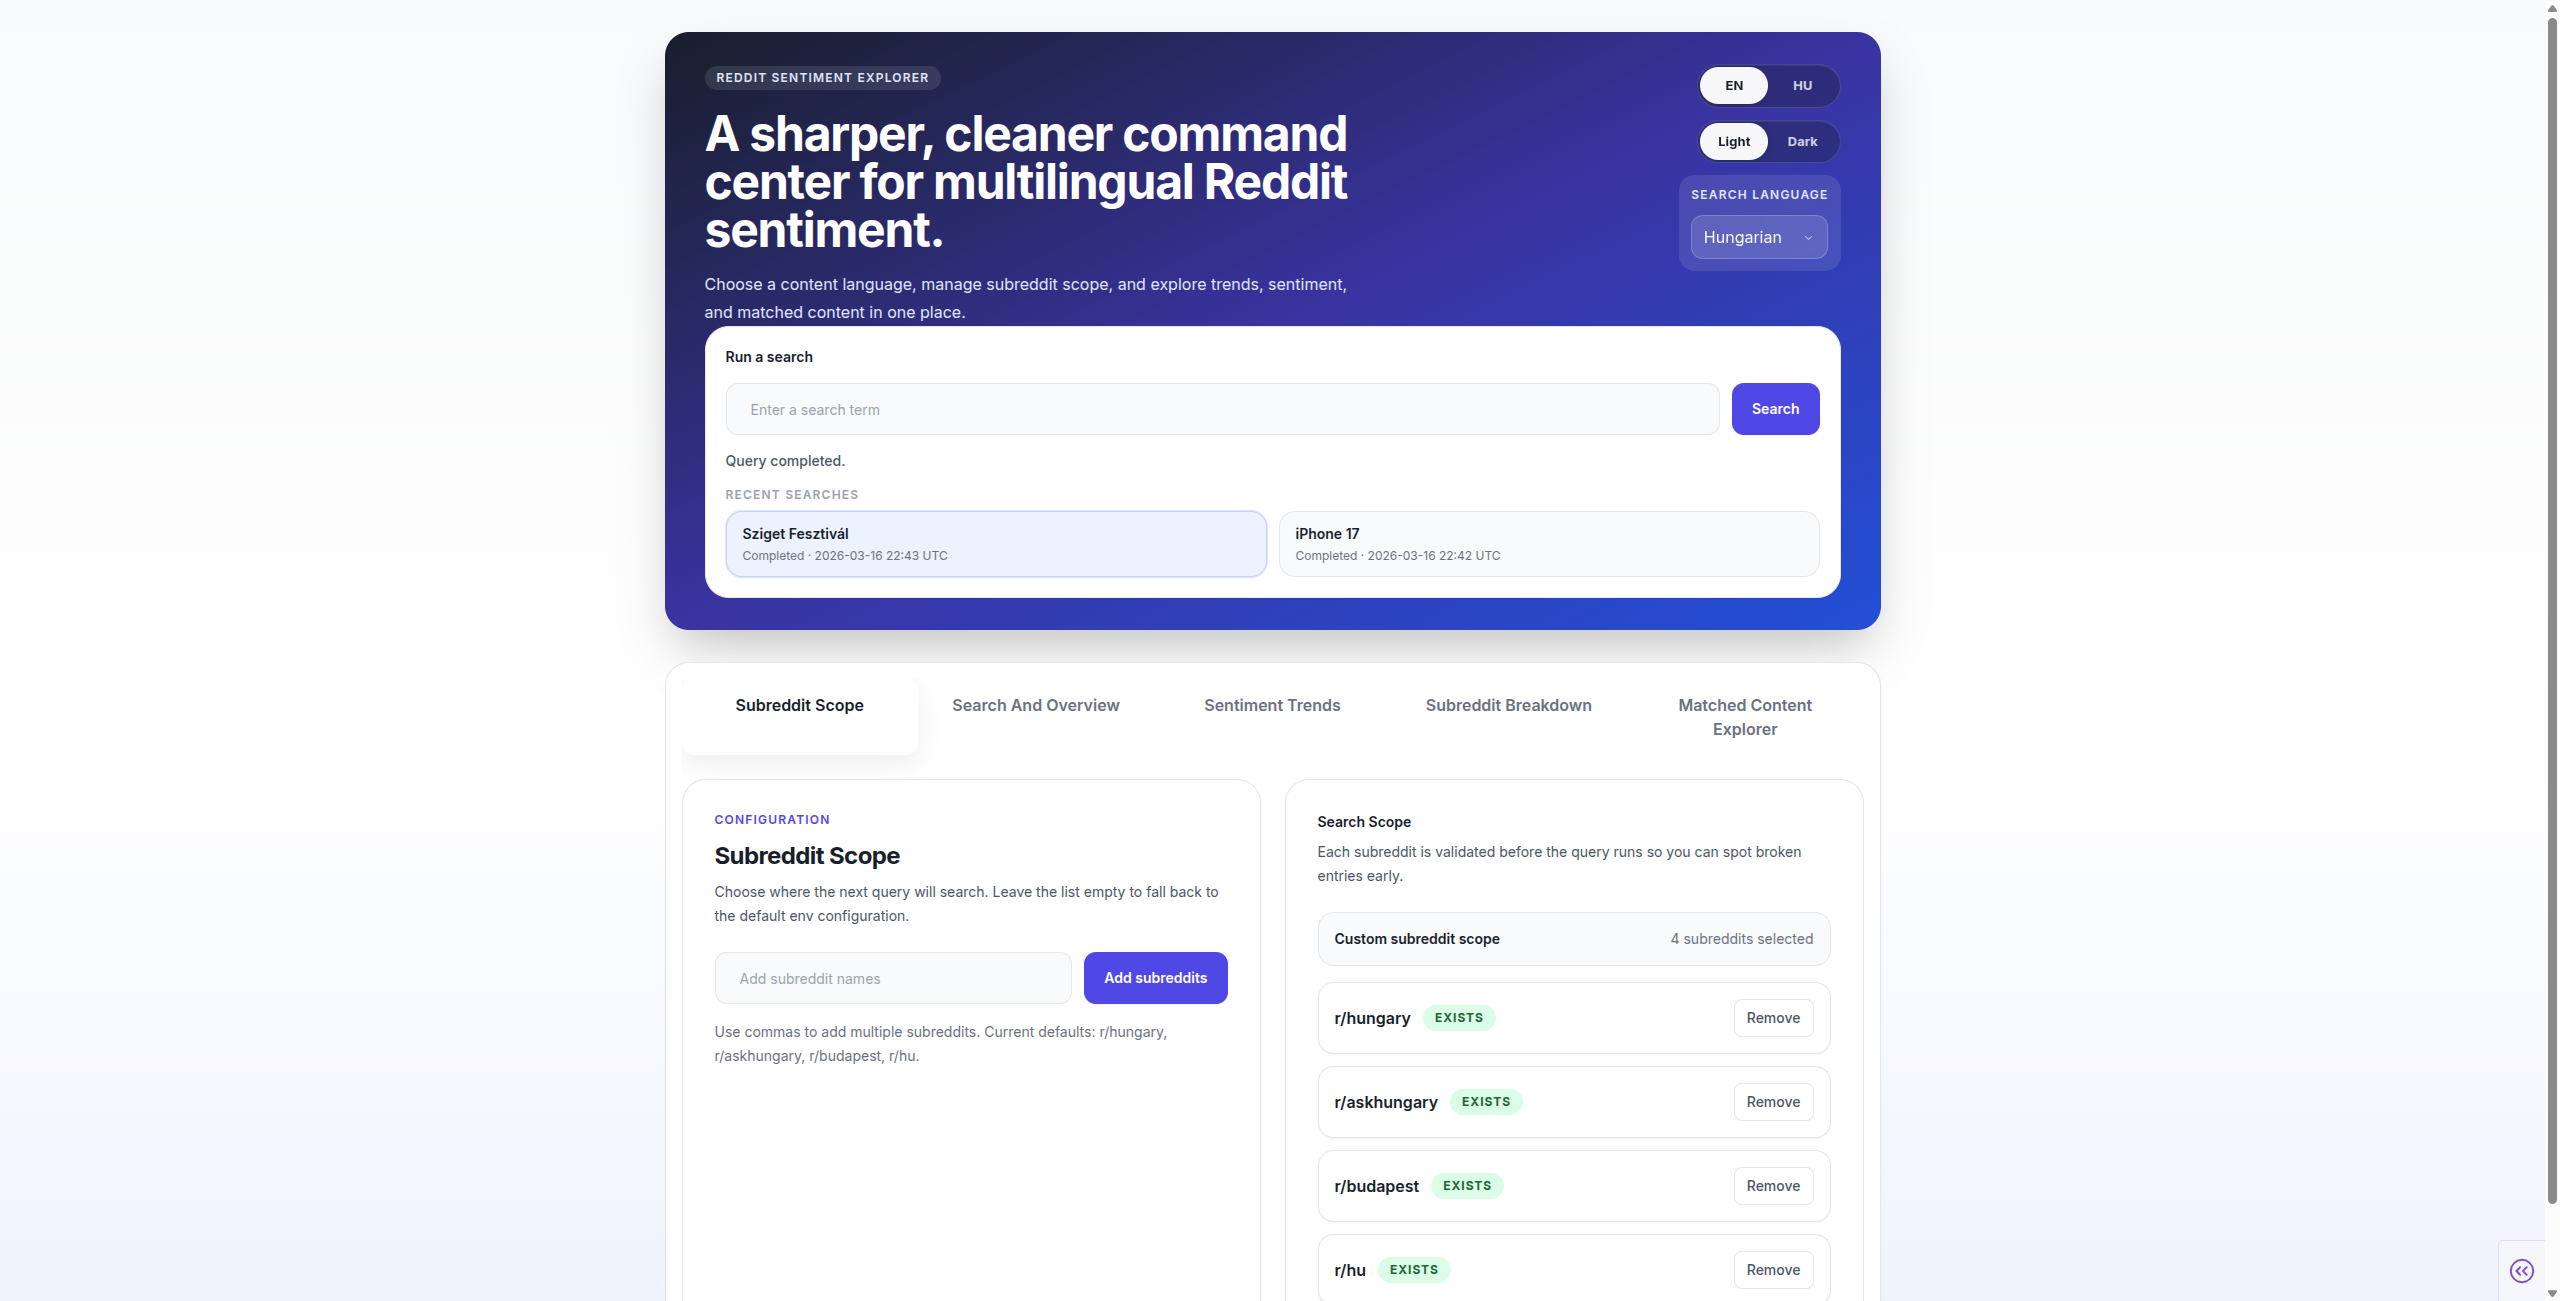
\includegraphics[width=\textwidth]{figures/dashboard-hero.png}
    \caption{Dashboard landing page with search interface and subreddit scope configuration. The left panel allows adding and removing subreddits, while the right panel shows the current scope with validation status.}
    \label{fig:dashboard_hero}
\end{figure}

The Subreddit Scope tab allows users to manage their search scope. Each subreddit is validated against the Reddit API when added, and its status is displayed as a badge. Users can add multiple subreddits at once using comma-separated names.

\subsection{Search Execution}
\label{sec:search_execution}

When the user types ``Sziget Fesztiv\'{a}l'' and clicks Search, the dashboard sends a POST request to the API, which creates a query and a query run. The dashboard then switches to the Search And Overview tab and begins polling the API every five seconds for status updates. A status message indicates that the query is being processed.

The worker picks up the pending run, marks it as running, and begins executing the pipeline: collecting posts and comments from Arctic Shift, matching and filtering content, classifying sentiment via the configured provider, and building aggregates.

\subsection{Search Overview Tab}

Once the pipeline completes, the dashboard displays the results on the Search And Overview tab. This tab provides four main views:

\begin{enumerate}
    \item \textbf{Overview metrics}: a summary card showing the total number of matched documents, the average sentiment score, the number of subreddits searched, and the count of higher- and lower-confidence classifications.
    \item \textbf{Sentiment timeline}: a line chart showing the average sentiment score per day, providing a temporal view of how sentiment evolves over time.
    \item \textbf{Rolling sentiment}: a smoothed seven-day rolling average of the sentiment score, which filters out daily noise and reveals longer-term trends.
    \item \textbf{Sentiment distribution}: a bar chart showing the count of documents in each of the five sentiment categories (very negative through very positive).
\end{enumerate}

Figure~\ref{fig:overview_metrics} shows the Search And Overview tab for the ``Sziget Fesztiv\'{a}l'' query. The overview metrics indicate 171 matched documents with an average sentiment score of $-0.69$, searched across 4 subreddits. The sentiment distribution reveals a predominantly negative skew: 86 documents classified as negative (50.3\%), 39 as neutral (22.8\%), 26 as very negative (15.2\%), and 20 as positive (11.7\%), with no documents classified as very positive. This distribution reflects the contentious nature of recent public discourse around the festival.

\begin{figure}[H]
    \centering
    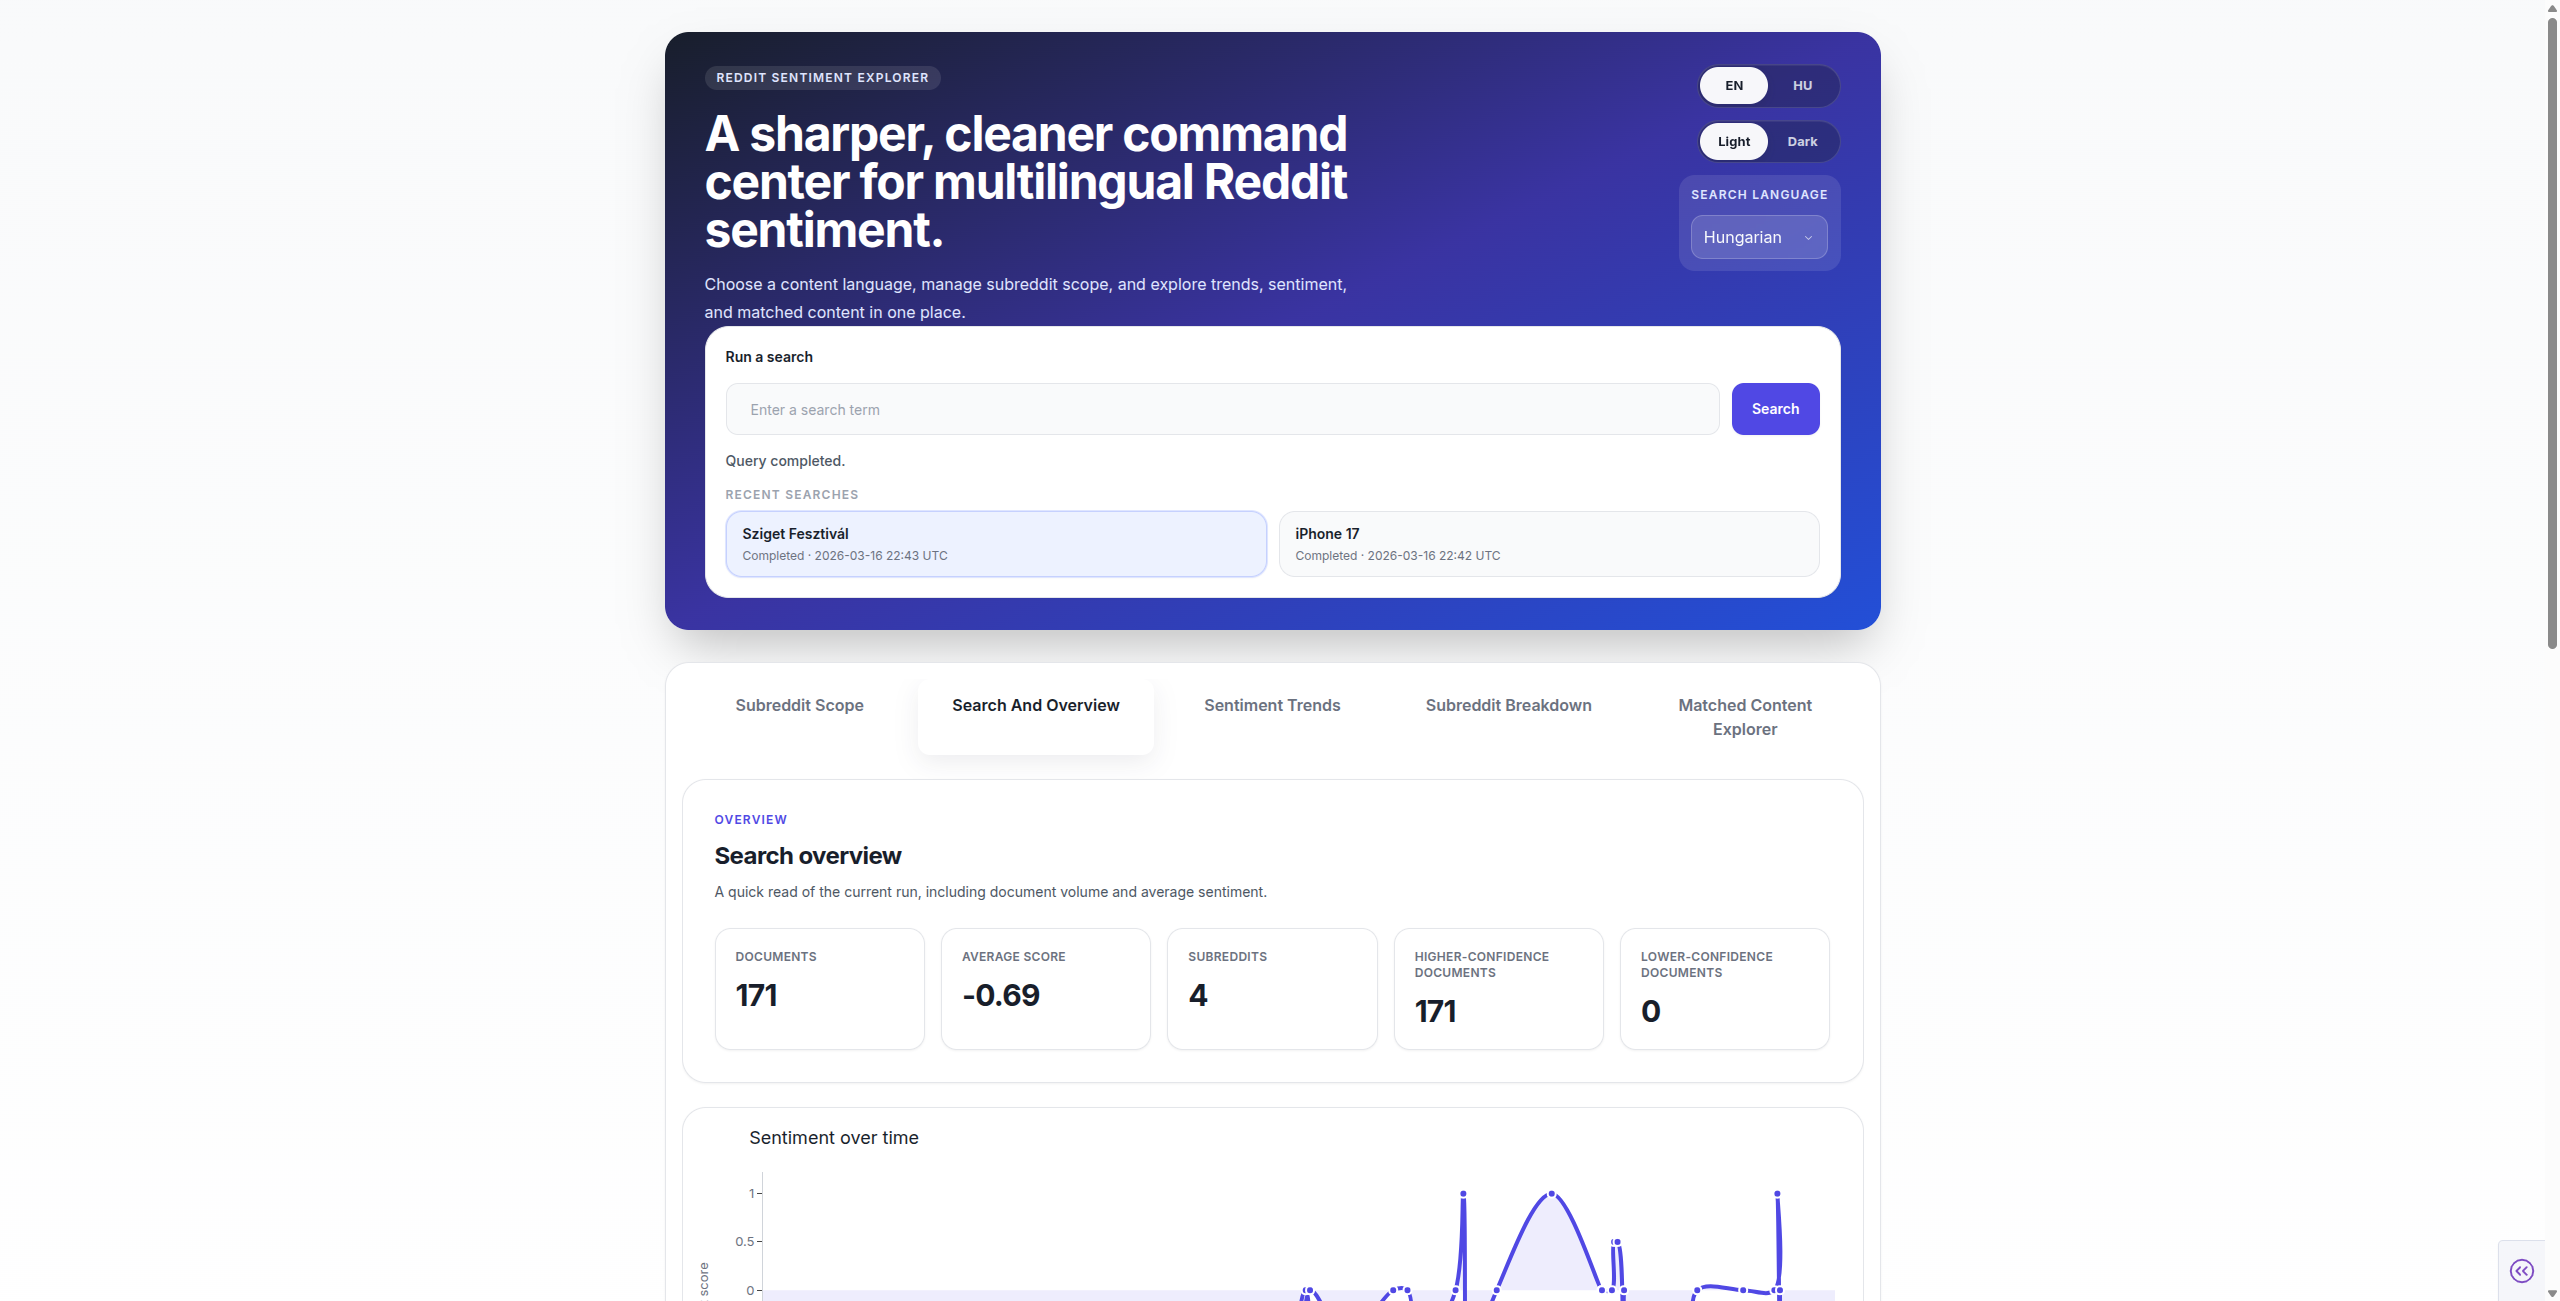
\includegraphics[width=\textwidth]{figures/overview-metrics.png}
    \caption{Search And Overview tab showing overview metrics and the beginning of the sentiment timeline for the ``Sziget Fesztiv\'{a}l'' query across four Hungarian subreddits.}
    \label{fig:overview_metrics}
\end{figure}

These views implement the overview+detail paradigm \cite{cockburn2008overview}. The user immediately sees the high-level picture: how many documents were found, whether overall sentiment is positive or negative, and how it varies over time.

\subsection{Sentiment Trends Tab}

The Sentiment Trends tab provides deeper temporal analysis with three charts:

\begin{enumerate}
    \item \textbf{Sentiment timeline}: same as the overview timeline but displayed at full width for detailed inspection.
    \item \textbf{Volume timeline}: a bar chart showing the number of documents per day, revealing how discussion volume fluctuates.
    \item \textbf{Sentiment heatmap}: a grid showing sentiment scores bucketed by date and subreddit. This reveals which communities discuss the search term and when, for example, showing that r/hungary dominates the conversation while r/askhungary and r/budapest contribute more sporadically.
\end{enumerate}

The content spans from March 2019 to December 2025, with a noticeable spike in discussion volume around late October 2025, when political debates about the festival's future intensified.

\begin{figure}[H]
    \centering
    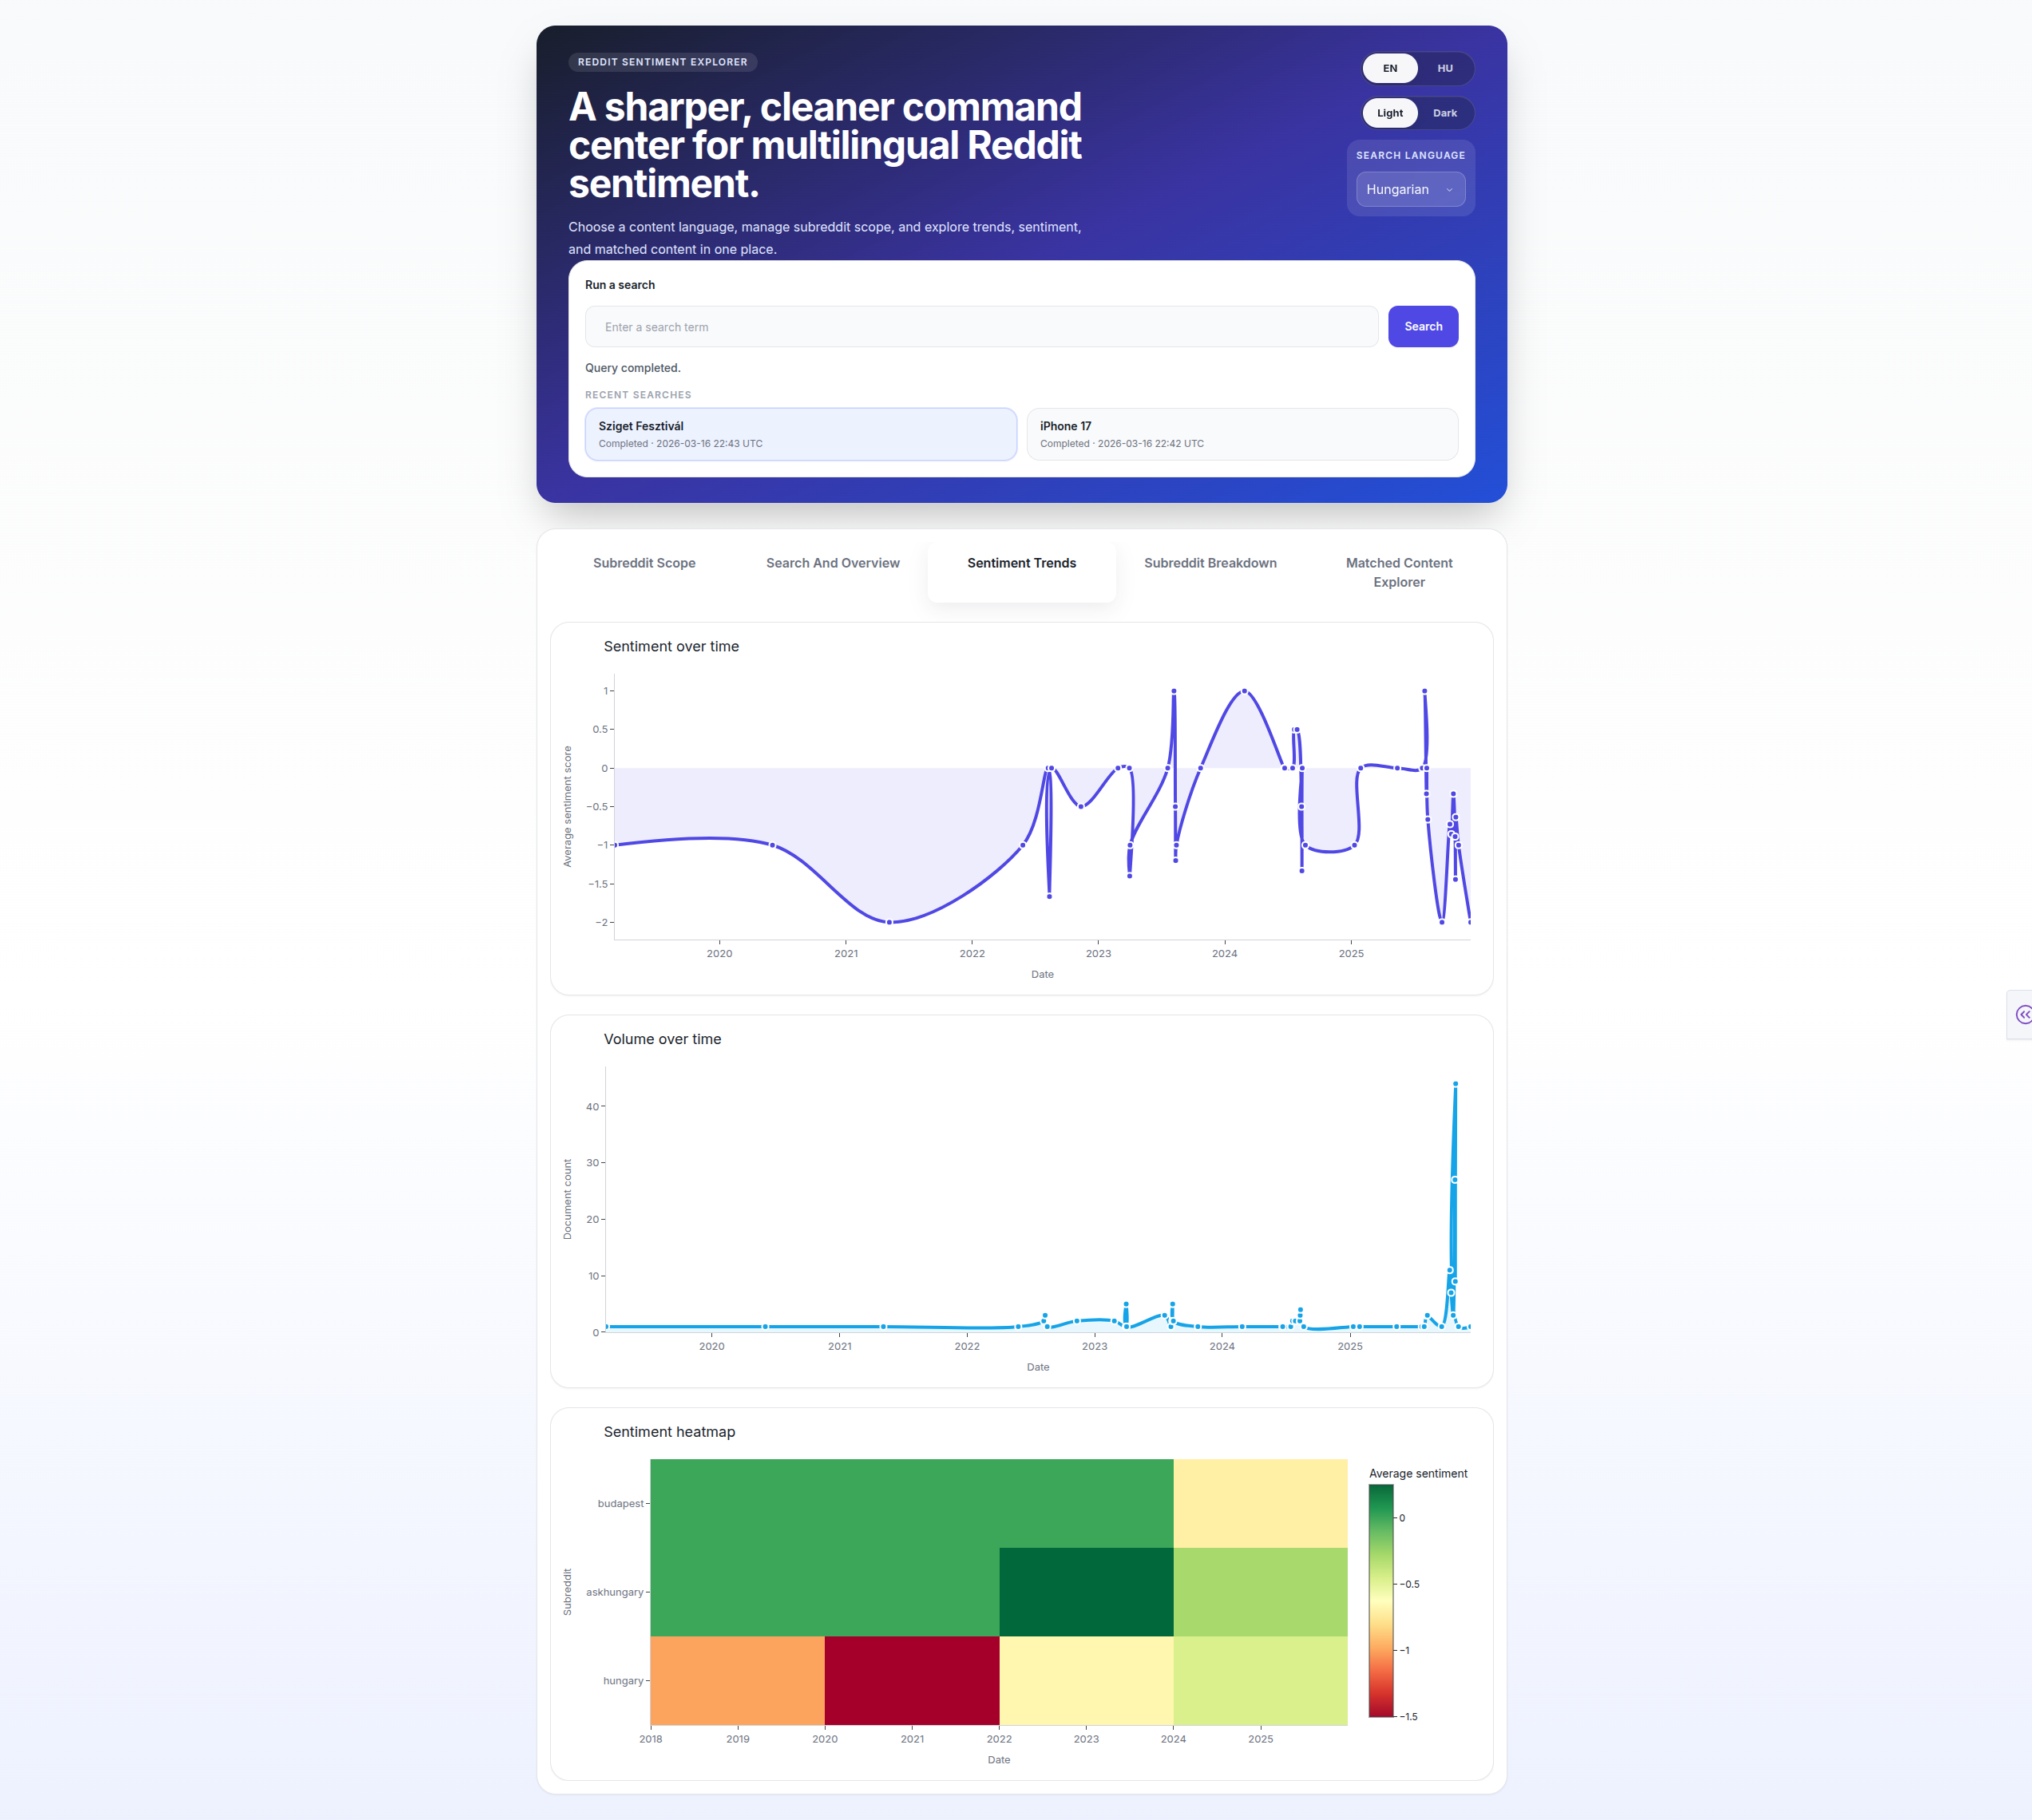
\includegraphics[width=\textwidth]{figures/sentiment-trends.png}
    \caption{Sentiment Trends tab showing the sentiment timeline, volume timeline, and sentiment heatmap for the ``Sziget Fesztiv\'{a}l'' query.}
    \label{fig:sentiment_trends}
\end{figure}

\subsection{Subreddit Breakdown Tab}

The Subreddit Breakdown tab enables comparative analysis across communities:

\begin{enumerate}
    \item \textbf{Subreddit chart}: a stacked bar chart showing the sentiment label distribution for each subreddit. The query returned content from three of the four subreddits: r/hungary (151 documents, average score $-0.75$), r/askhungary (13 documents, average score $0.00$), and r/budapest (7 documents, average score $-0.57$). The r/hu subreddit returned no matching content.
    \item \textbf{Phrase drivers}: evidence phrases grouped by sentiment label, revealing the most common themes. For example, the positive bucket highlights ``j\"{o}v\H{o}re tal\'{a}lkozunk a fesztiv\'{a}lon'' (see you next year at the festival), while the very negative bucket features ``s\'{u}lyos presztizsvesztes\'{e}get'' (serious prestige loss) and ``gyeng\'{\i}ten\'{e} az orsz\'{a}g turisztikai'' (would weaken the country's tourism).
    \item \textbf{Spike events}: a list of dates with unusually high document volume or extreme sentiment, helping users identify specific events that drove discussion.
\end{enumerate}

\begin{figure}[H]
    \centering
    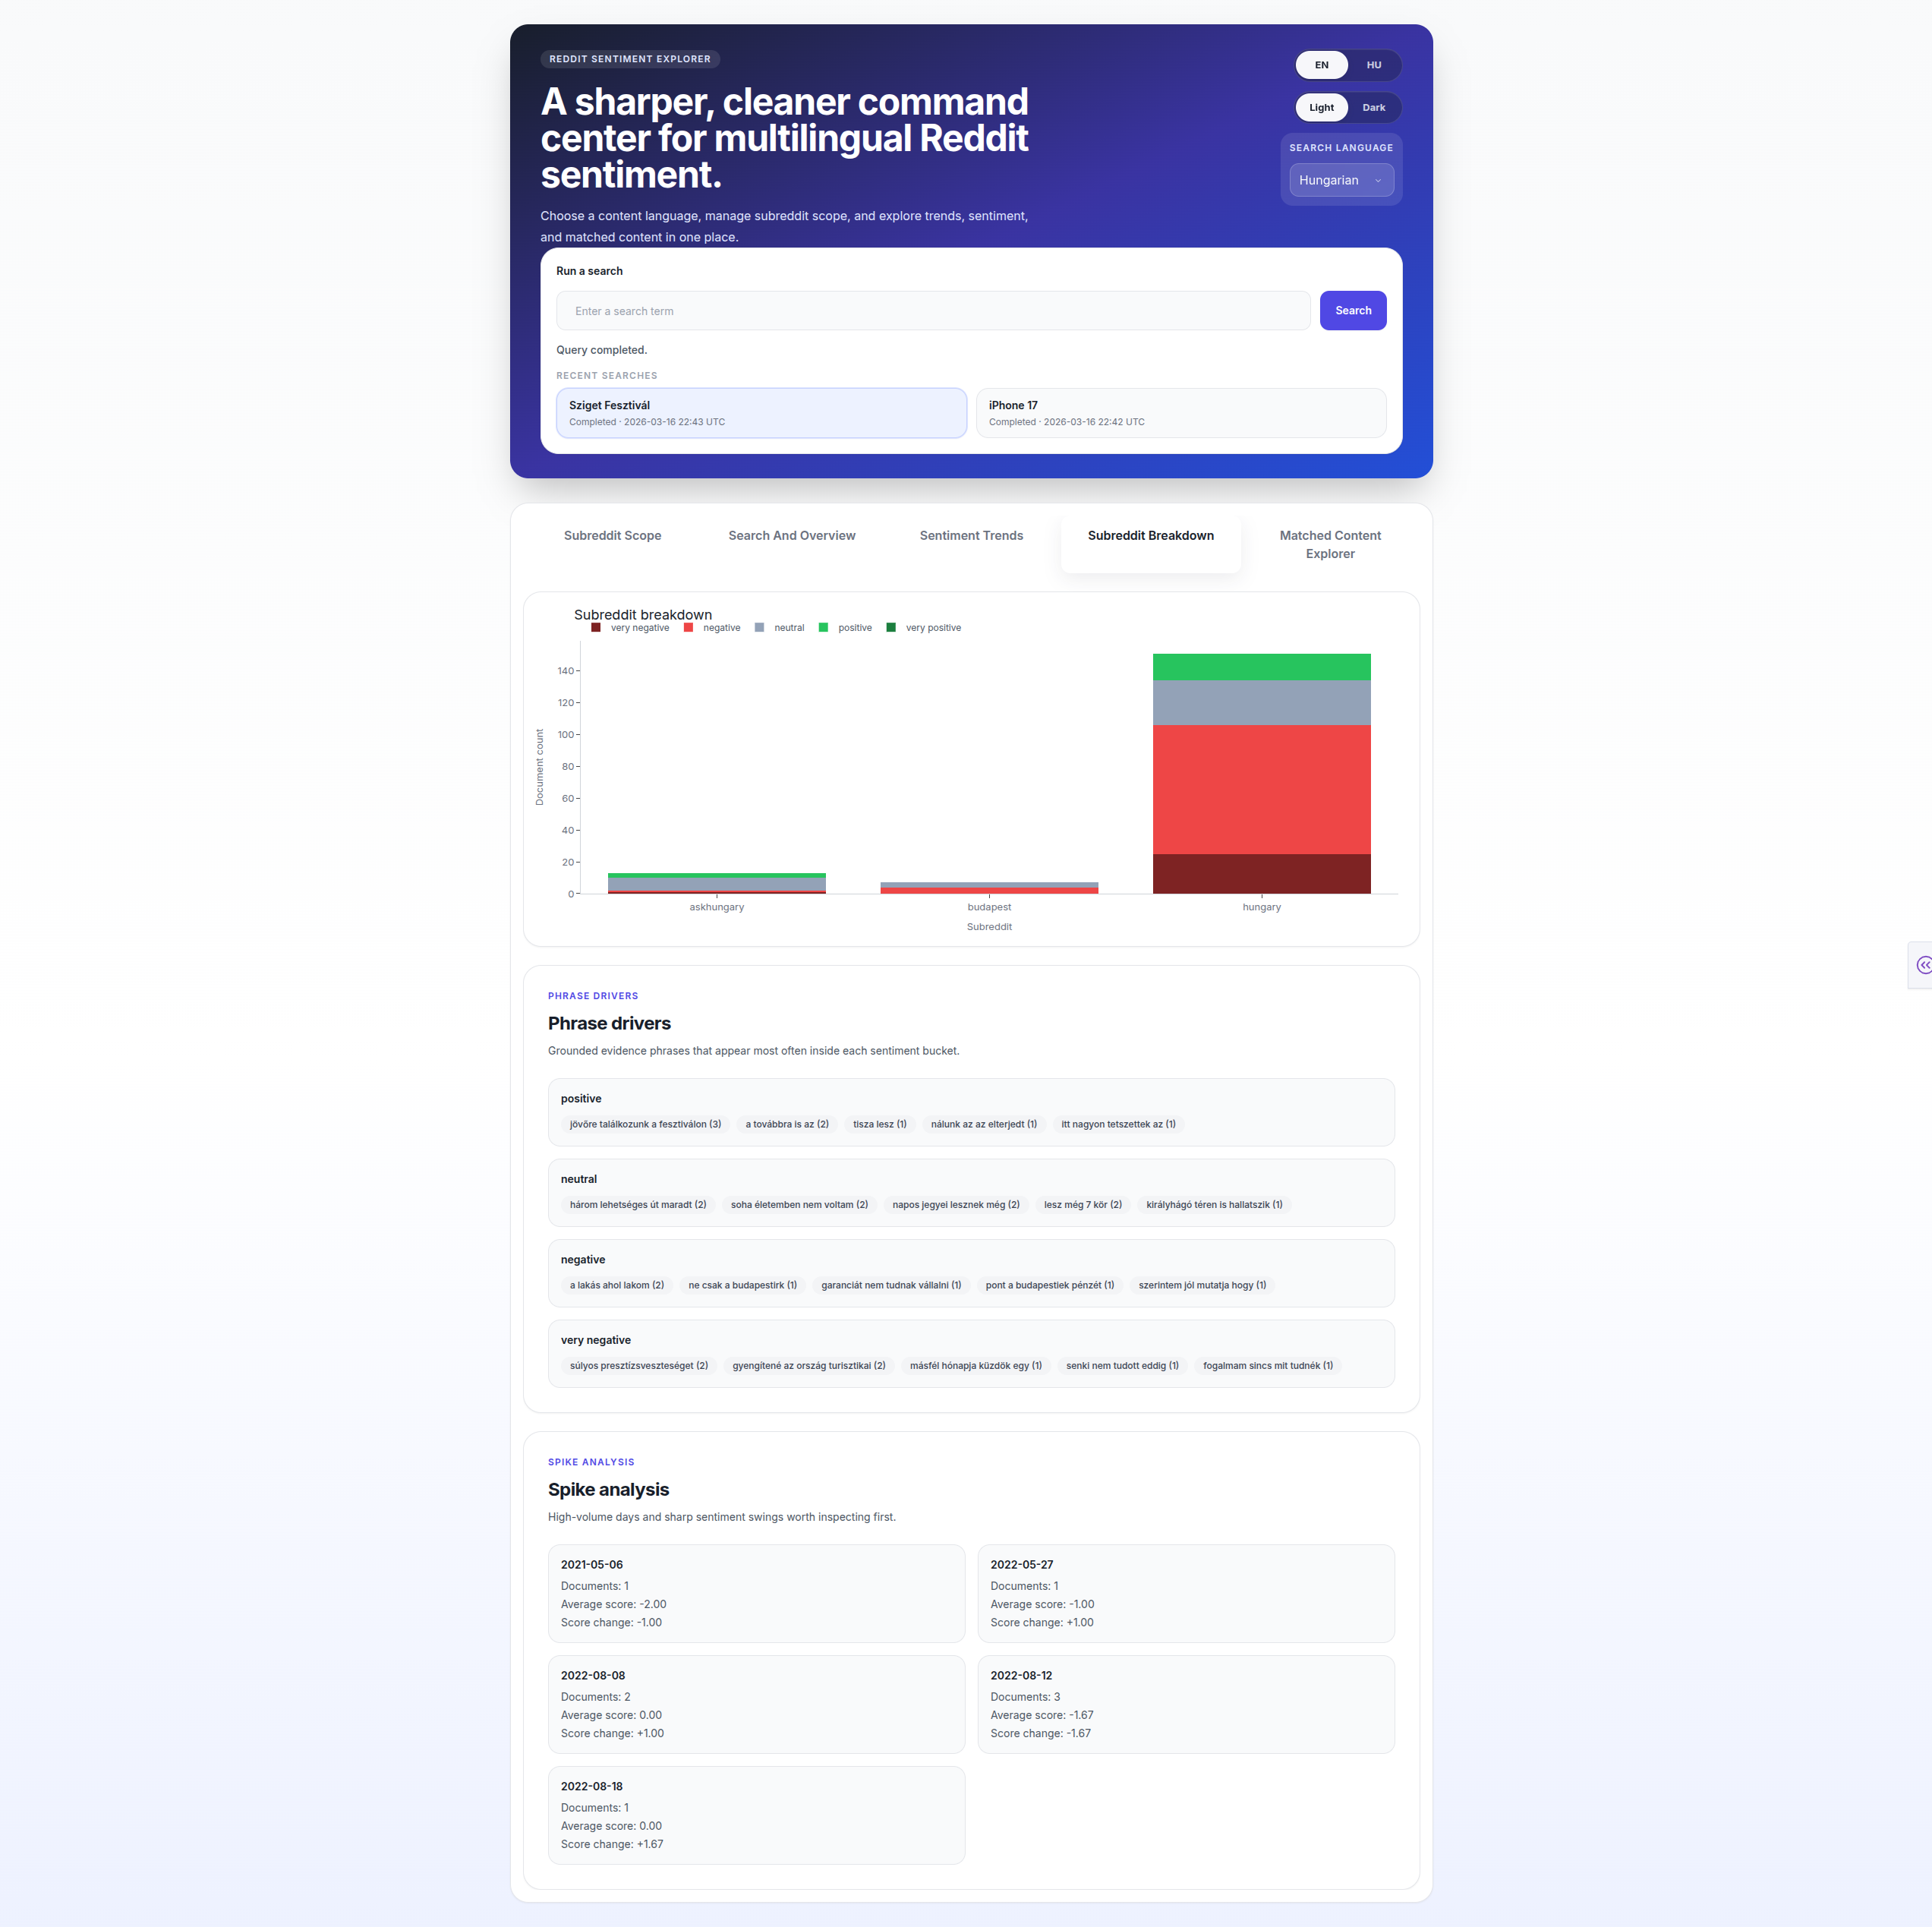
\includegraphics[width=\textwidth]{figures/subreddit-breakdown.png}
    \caption{Subreddit Breakdown tab showing the per-subreddit sentiment distribution, phrase drivers grouped by sentiment label, and spike analysis with notable dates.}
    \label{fig:subreddit_breakdown}
\end{figure}

\subsection{Matched Content Explorer}

The Matched Content Explorer tab provides the ``details on demand'' layer. It lists all matched documents with their sentiment label, source type, date, and a text preview. Users can filter by date, subreddit, sentiment, and source type, or search within the snippet text. Clicking any row expands its full details, including:

\begin{itemize}
    \item The complete text of the post or comment.
    \item The sentiment label and numeric score.
    \item The confidence level of the classification.
    \item The rationale explaining why the model assigned this label.
    \item Evidence phrases: exact quotes from the text that support the classification.
    \item A link to the original Reddit post or comment.
\end{itemize}

Figure~\ref{fig:matched_content} shows the Matched Content Explorer filtered to positive documents, with a selected comment that reads: ``Sosem voltam a Szigeten, mert nem nekem val\'{o} zen\'{e}k vannak ott, de tagadhatatlan, hogy eg\'{e}sz Eur\'{o}p\'{a}ban az egyik legnagyobb zenei fesztiv\'{a}l'' (I've never been to Sziget because the music isn't my style, but it's undeniable that it's one of the largest music festivals in all of Europe). The model classified this as positive with 0.85 confidence, with the rationale noting that the text highlights the festival's positive impact despite the author's personal preferences. The evidence phrases quote passages about the festival being one of the largest in Europe, visitors spending money and enjoying themselves, and Budapest being one of Europe's most beautiful cities.

\begin{figure}[H]
    \centering
    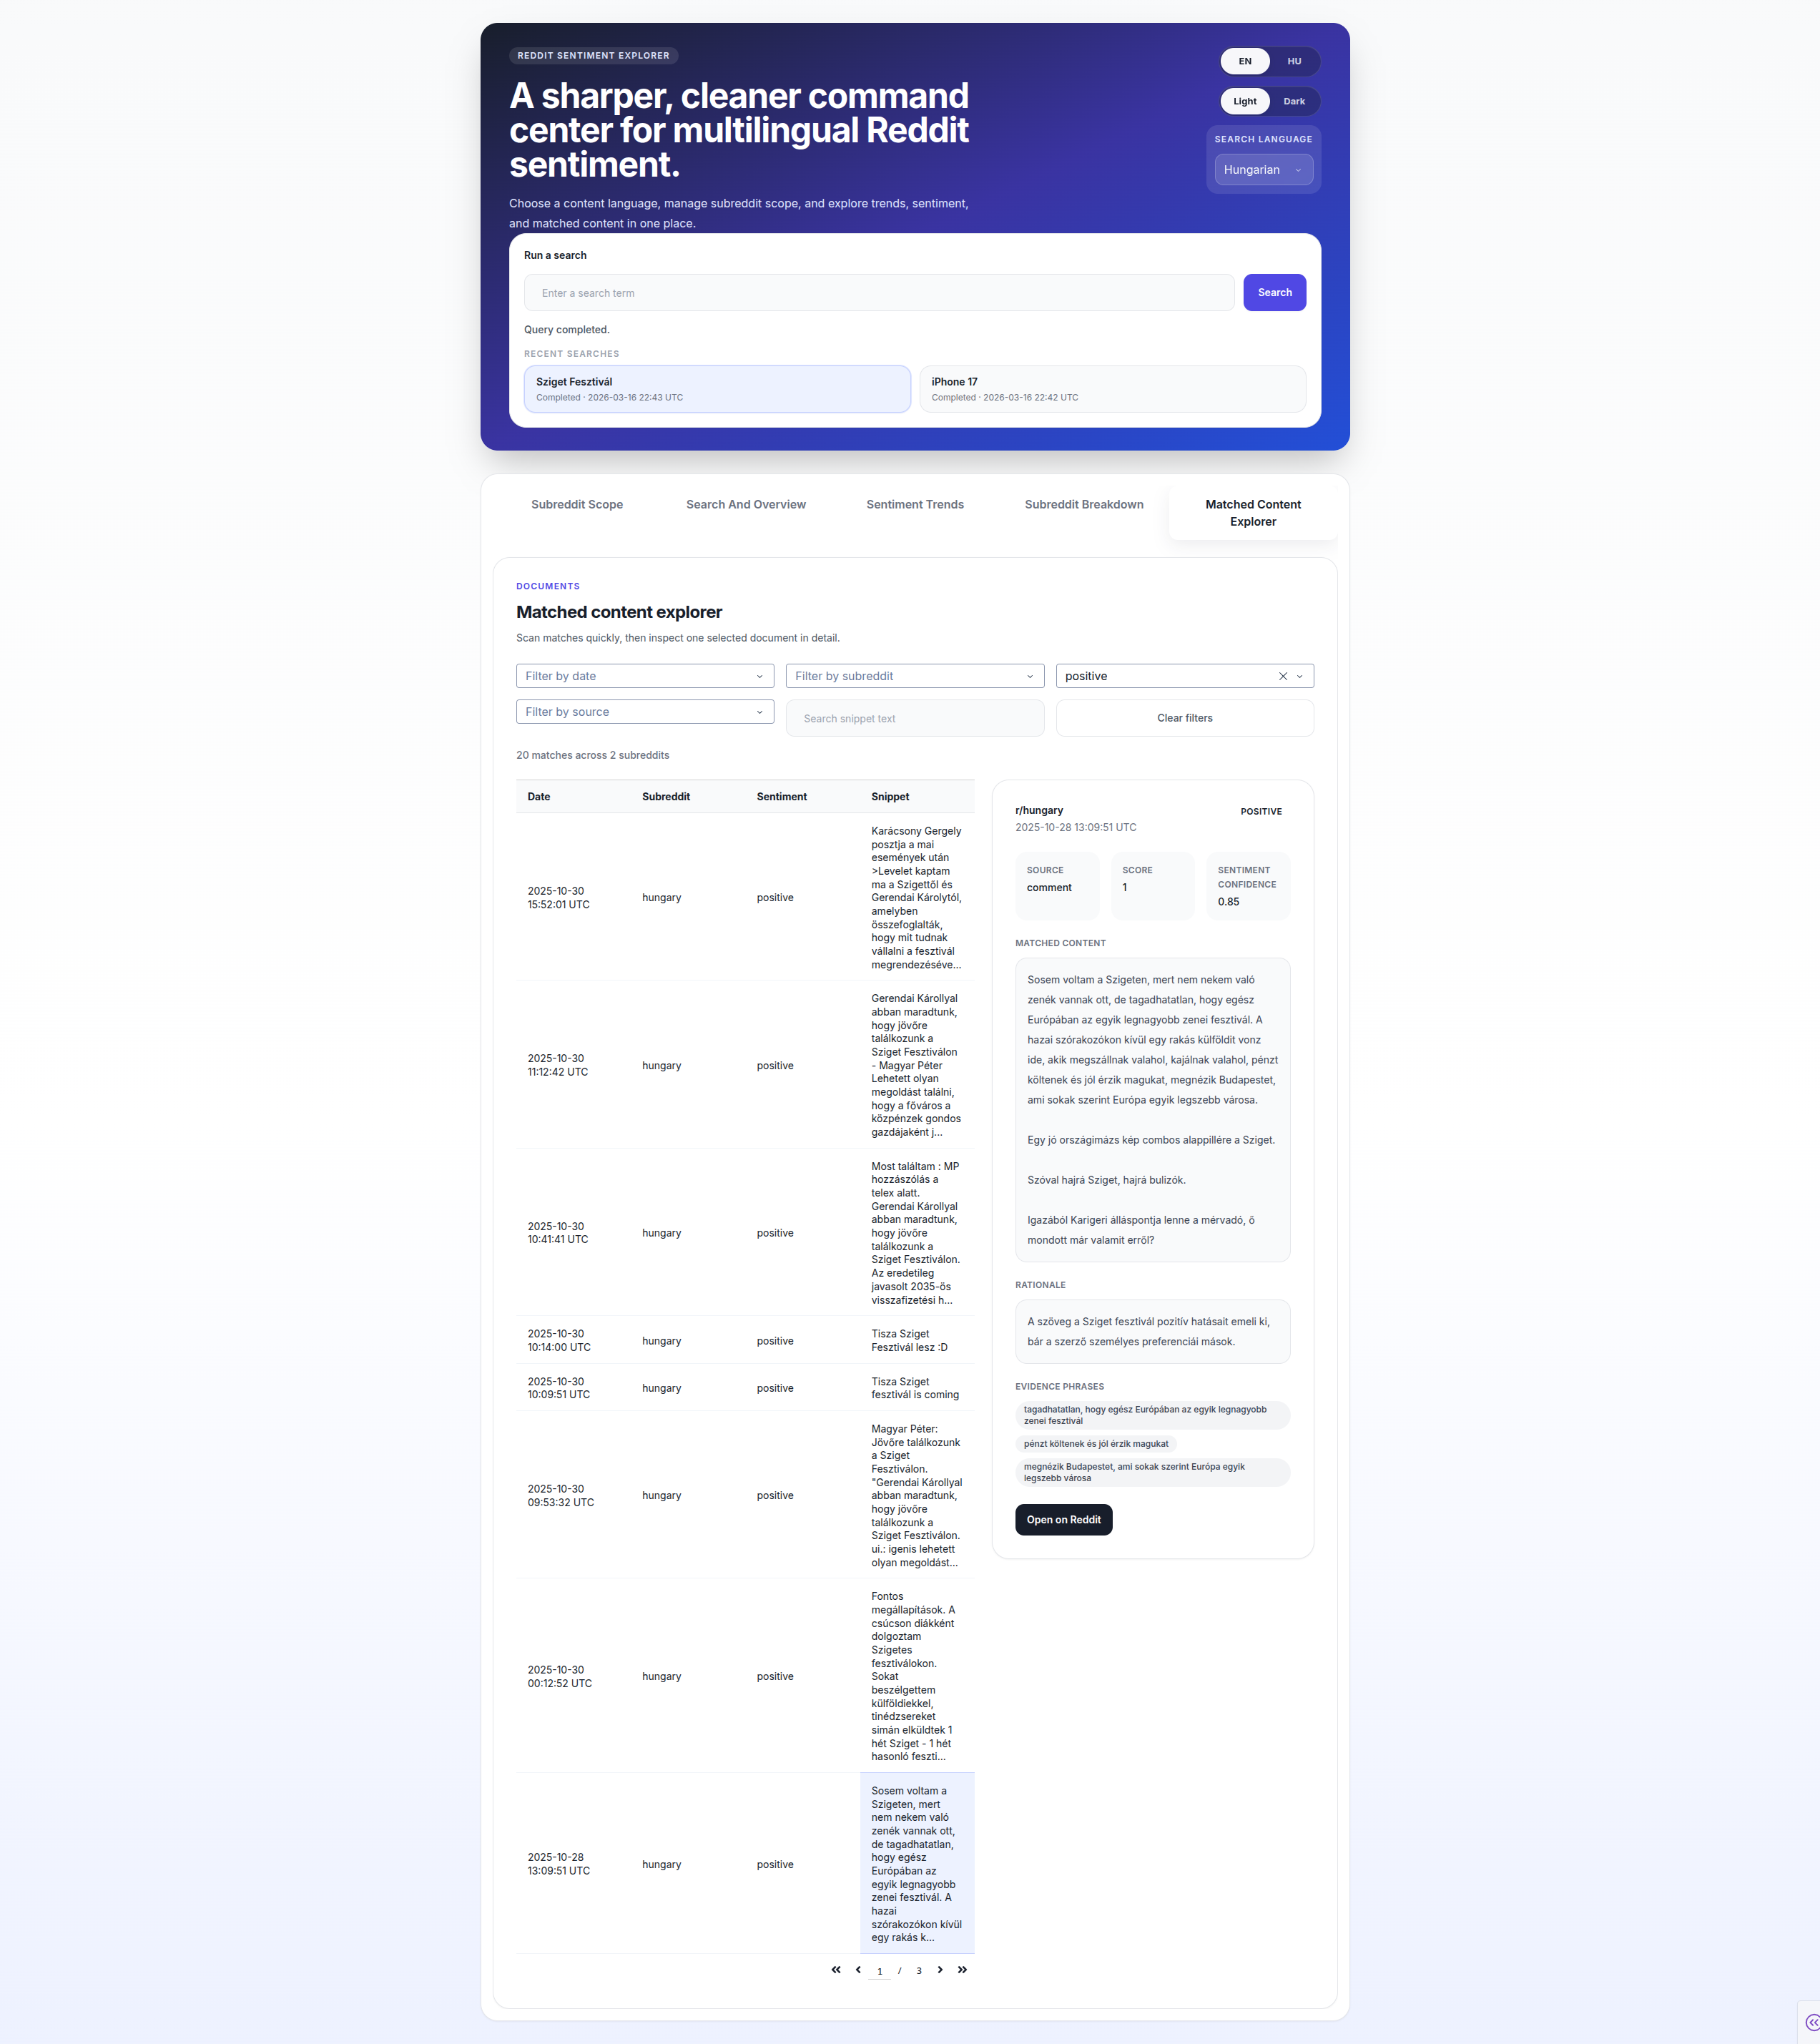
\includegraphics[width=\textwidth]{figures/matched-content.png}
    \caption{Matched Content Explorer filtered to positive documents, showing a comment classified as positive with the rationale in Hungarian and evidence phrases extracted from the source text.}
    \label{fig:matched_content}
\end{figure}

This example demonstrates the model's ability to look beyond surface-level cues: the author explicitly states they have never attended the festival, yet the overall tone is supportive. A keyword-based classifier would struggle to determine sentiment from this text, whereas the LLM correctly identifies the positive framing.

\section{Sentiment Classification Quality}
\label{sec:classification_quality}

I evaluate the sentiment classification quality by examining the outputs of the OpenAI provider and comparing them with the mock provider.

\subsection{OpenAI Provider Strengths}

The OpenAI provider (using GPT-4o-mini) demonstrates several strengths in classifying Reddit content:

\begin{enumerate}
    \item \textbf{Context understanding.} The model understands implicit sentiment, sarcasm, and opinions embedded in longer narratives. For example, a comment that begins with a personal disclaimer (``I've never been there'') but proceeds to praise the festival's economic and cultural value is correctly classified as positive.

    \item \textbf{Multilingual capability.} All 171 documents in this query were detected as Hungarian, and the model classified them without requiring a separate model or translation step. The rationale is provided in Hungarian when the input is Hungarian, making it accessible to the end user.

    \item \textbf{Interpretable output.} The rationale and evidence phrases provide transparency into the classification decision. This is a substantial improvement over traditional classifiers that output only a label and a probability.

    \item \textbf{Fine-grained discrimination.} The model distinguishes between ``negative'' and ``very negative,'' capturing the intensity of sentiment. A comment expressing mild disappointment about ticket prices is classified as negative, while a text describing ``serious prestige loss'' and ``weakening the country's tourism brand'' receives a very negative label with 0.95 confidence.
\end{enumerate}

\subsection{OpenAI Provider Limitations}

\begin{enumerate}
    \item \textbf{Non-determinism.} The same text may receive different labels across runs due to the stochastic nature of language model generation. While the system mitigates this through result caching (the same document is only classified once per provider), different query runs may produce slightly different aggregate statistics for the same content.

    \item \textbf{Cost.} Each classification requires an API call, which incurs a cost. For a query that matches 171 documents, the cumulative cost is noticeable. The current implementation processes documents sequentially, which also contributes to pipeline execution time.

    \item \textbf{Latency.} Each API call takes approximately 0.5--2 seconds, depending on input length and model load. For a query with 171 matched documents, classification alone can take 2--5 minutes.

    \item \textbf{Occasional format errors.} Despite the structured JSON output format, the model occasionally returns confidence as a string (``high'' instead of 0.8) or omits fields. The implementation handles these cases through a confidence normalization method and default values.
\end{enumerate}

\subsection{Comparison with Mock Provider}

The mock provider uses word-counting heuristics and serves as a baseline. It is fast (instant classification) and free (no API costs), but has clear limitations:

\begin{itemize}
    \item It cannot detect sarcasm, irony, or implicit sentiment.
    \item It treats all occurrences of positive/negative words equally regardless of context.
    \item Its word lists are limited and do not cover domain-specific vocabulary.
    \item It assigns fixed confidence values (0.5--0.6) regardless of the actual ambiguity of the text.
\end{itemize}

In informal testing on Hungarian Reddit content, the OpenAI provider produced more nuanced and contextually appropriate results. The mock provider tended to classify most content as neutral due to the limited Hungarian word list, while the OpenAI provider identified a wider range of sentiment intensities.

\section{System Performance}
\label{sec:performance}

\subsection{Pipeline Throughput}

The end-to-end pipeline time depends primarily on two factors: the number of documents collected and the speed of sentiment classification. Data collection from Arctic Shift typically takes 5--15 seconds depending on the number of subreddits and the volume of matching content. Sentiment classification with the OpenAI provider dominates the execution time, processing documents sequentially at 0.5--2 seconds per document.

For the ``Sziget Fesztiv\'{a}l'' query, the pipeline collected 59 posts and 112 comments across three subreddits, classified all 171 matched documents, and built nine types of aggregates. The complete pipeline execution took approximately three minutes.

\subsection{Caching Effectiveness}

The TTL-based caching strategy (default 12 hours) effectively eliminates redundant pipeline executions. Repeated queries for the same term, subreddit scope, and language return cached results instantly. The cache hit rate depends on usage patterns; in a scenario where multiple users explore the same topics, caching provides substantial time and cost savings.

\subsection{Database Performance}

PostgreSQL handles the workload efficiently for the scale of this application. The \texttt{FOR UPDATE SKIP LOCKED} pattern for worker task claiming adds minimal overhead. Precomputed aggregates ensure that chart rendering requires only a single row lookup per aggregate type, regardless of the number of underlying documents.

\section{Discussion}
\label{sec:discussion}

\subsection{Addressing the Research Questions}

\textbf{Research Question 1: How can a modular, query-driven system be designed to collect, filter, and classify Reddit content by sentiment?}

The implementation demonstrates that a four-service architecture with a clear pipeline of stages (collect, persist, match, filter, classify, aggregate) achieves the goal. The separation of concerns enables each component to be developed, tested, and modified independently. The provider abstraction makes sentiment classification pluggable. The Document entity provides a clean abstraction layer between Reddit-specific data and the classification pipeline. The caching strategy and background worker pattern keep the user interface responsive despite long-running classification tasks.

\textbf{Research Question 2: How effectively can large language models classify sentiment in informal, multilingual social media text?}

The ``Sziget Fesztiv\'{a}l'' case study demonstrates that GPT-4o-mini correctly handles Hungarian-language informal text, including political commentary, sarcasm, and nuanced opinions. The model produced interpretable, contextually appropriate classifications across all 171 documents, with high confidence scores (all above the lower-confidence threshold). The rationale and evidence phrases, provided in the language of the source text, add a layer of transparency that traditional classifiers do not offer. The trade-offs (non-determinism, per-call cost, latency) are acceptable for a query-driven exploration tool but would require mitigation for high-volume production use.

\subsection{Comparison with Existing Approaches}

\begin{sloppypar}
Compared to the fragmented scripting approach common in academic research, Reddit Sentiment Explorer provides an integrated, interactive experience from search to visualization. Compared to commercial social listening platforms, it is open-source, customizable, and supports arbitrary search terms without predefined topic constraints. The main limitation relative to commercial tools is scalability: the current single-worker architecture is suited for individual exploration rather than large-scale enterprise monitoring.
\end{sloppypar}

\chapter{Conclusions}
\label{ch:conclusions}

This chapter summarizes the contributions of the thesis, discusses the limitations of the current implementation, and outlines directions for future work.

\section{Summary}
\label{sec:summary}

In this thesis, I designed and implemented Reddit Sentiment Explorer, a query-driven web platform for analyzing public opinion on Reddit using large language models. The system enables users to enter any search term, select target subreddits and a content language, and receive comprehensive sentiment analysis results through an interactive dashboard.

The platform addresses the gap between ad-hoc sentiment analysis scripts and commercial social listening platforms by providing an integrated, open-source tool that handles the complete workflow from data collection to interactive visualization. The key contributions are:

\begin{enumerate}
    \item \textbf{A modular, four-service architecture} that cleanly separates the API, worker, dashboard, and database concerns. This architecture enables independent development and deployment of each component, and the pipeline design (collect, persist, match, filter, classify, aggregate) provides clear extension points for future enhancements.

    \item \textbf{A provider-agnostic sentiment classification layer} that abstracts the classification interface behind a Python protocol. This enables swapping between an OpenAI-based provider for production use and a heuristic mock provider for development, and can accommodate new providers (such as open-source models) without changes to the rest of the system.

    \item \textbf{Interpretable sentiment classification} that goes beyond labels and confidence scores. By leveraging the language generation capabilities of large language models, each classification includes a rationale and evidence phrases, making the results transparent and verifiable by the end user.

    \item \textbf{A document abstraction layer} that normalizes Reddit posts and comments into a common representation. This simplifies the matching, classification, and aggregation logic and makes the pipeline agnostic to the underlying content type.

    \item \textbf{An interactive dashboard} with nine types of aggregated visualizations (overview, distribution, timelines, heatmaps, breakdowns, spike detection), multilingual UI support (English and Hungarian), and light/dark themes. The dashboard follows the Visual Information Seeking Mantra, providing overview first, then zoom and filter, then details on demand.
\end{enumerate}

The evaluation demonstrates that the OpenAI provider produces contextually appropriate, multilingual sentiment classifications on informal Reddit text, with interpretable output that traditional classifiers do not provide. The system successfully answers both research questions posed in Chapter~\ref{ch:introduction}.

\section{Limitations}
\label{sec:limitations}

Several limitations should be acknowledged:

\begin{enumerate}
    \item \textbf{Data freshness.} The Arctic Shift archive provides historical Reddit data but may not include the most recent posts and comments. This means the platform is better suited for retrospective analysis than real-time monitoring.

    \item \textbf{Classification cost and latency.} The OpenAI provider requires a paid API key and processes documents sequentially, resulting in execution times of 1--3 minutes for queries with many matched documents. This limits the platform's suitability for high-volume or time-sensitive use cases.

    \item \textbf{Single-worker throughput.} The current architecture uses a single worker process. While the \texttt{FOR UPDATE SKIP LOCKED} pattern supports multiple concurrent workers, horizontal scaling has not been tested.

    \item \textbf{Non-deterministic classification.} Large language model outputs are inherently non-deterministic. The same document may receive different labels across separate classification runs, which can affect the reproducibility of aggregate statistics.

    \item \textbf{Limited evaluation scope.} The sentiment classification quality was evaluated through qualitative inspection rather than a formal evaluation against a labeled dataset. Constructing a gold-standard dataset for fine-grained, multilingual Reddit sentiment classification was beyond the scope of this thesis.

    \item \textbf{Language detection accuracy.} The \texttt{langdetect} library performs well on longer texts but is less reliable on short Reddit comments (one or two sentences), which can lead to both false positives and false negatives in language filtering.
\end{enumerate}

\section{Future Work}
\label{sec:future_work}

Several directions could extend the platform:

\begin{enumerate}
    \item \textbf{Multi-provider sentiment ensemble.} Running multiple providers (e.g., OpenAI, a fine-tuned BERT model, and a lexicon-based approach) and aggregating their predictions could improve both accuracy and robustness while providing a confidence measure based on inter-provider agreement.

    \item \textbf{Real-time streaming.} Integrating with Reddit's real-time data sources or more frequently updated archives would enable monitoring of emerging discussions as they happen.

    \item \textbf{Concurrent classification.} Processing documents in parallel (batched API calls or concurrent workers) would significantly reduce pipeline execution time for large queries.

    \item \textbf{Open-source model support.} Adding providers for locally hosted models (e.g., Llama, Mistral) would eliminate API costs and provide full data privacy, which is important for sensitive analysis topics.

    \item \textbf{Broader platform support.} Extending the collector abstraction to support additional platforms (Twitter/X, HackerNews, news websites) would make the tool applicable to cross-platform sentiment analysis.

    \item \textbf{User accounts and saved queries.} Adding authentication and persistent user profiles would enable saved query histories, scheduled recurring analyses, and collaborative use.

    \item \textbf{Formal evaluation framework.} Building a labeled evaluation dataset of Reddit content across multiple languages and domains would enable rigorous quantitative comparison of sentiment providers.
\end{enumerate}

Reddit Sentiment Explorer demonstrates that combining modern web technologies with large language model capabilities produces a practical tool for exploratory sentiment analysis. The modular architecture and provider abstraction ensure that as both web technologies and language models continue to evolve, the platform can adapt without fundamental restructuring.


\bibliography{references}

\newpage
\appendix
\pagestyle{fancy}
\fancyhf{}
\fancyhead[R]{Appendices}
\renewcommand{\headrulewidth}{0.4pt}

\section*{Appendix A: Database Schema}

Table~\ref{tab:schema_queries} through Table~\ref{tab:schema_aggregates} document the complete database schema used by the application.

\begin{table}[H]
\centering
\caption{queries table}
\label{tab:schema_queries}
\small
\begin{tabularx}{\textwidth}{ll>{\raggedright\arraybackslash}X}
\toprule
\textbf{Column} & \textbf{Type} & \textbf{Description} \\
\midrule
id & VARCHAR(36) PK & UUID primary key \\
raw\_term & VARCHAR(255) & Original search term as entered by user \\
normalized\_term & VARCHAR(255) UNIQUE & Lowercased, accent-stripped, whitespace-collapsed \\
created\_at & TIMESTAMP & Creation timestamp \\
\bottomrule
\end{tabularx}
\end{table}

\begin{table}[H]
\centering
\caption{query\_runs table}
\label{tab:schema_query_runs}
\small
\begin{tabularx}{\textwidth}{ll>{\raggedright\arraybackslash}X}
\toprule
\textbf{Column} & \textbf{Type} & \textbf{Description} \\
\midrule
id & VARCHAR(36) PK & UUID primary key \\
query\_id & VARCHAR(36) FK & Reference to queries table \\
status & ENUM & pending, running, completed, failed \\
started\_at & TIMESTAMP & When the run was created \\
finished\_at & TIMESTAMP & When the run completed or failed \\
scope\_config & JSON & Subreddit list and other scope parameters \\
match\_strategy & VARCHAR(100) & Matching strategy name \\
language\_filter & VARCHAR(50) & Target content language code \\
data\_fresh\_until & TIMESTAMP & Cache expiry timestamp \\
error\_message & TEXT & Error details if status is failed \\
\bottomrule
\end{tabularx}
\end{table}

\begin{table}[H]
\centering
\caption{documents table}
\label{tab:schema_documents}
\small
\begin{tabularx}{\textwidth}{ll>{\raggedright\arraybackslash}X}
\toprule
\textbf{Column} & \textbf{Type} & \textbf{Description} \\
\midrule
id & VARCHAR(36) PK & UUID primary key \\
source\_type & ENUM & post or comment \\
source\_id & VARCHAR(36) & ID of the source post or comment \\
subreddit\_id & VARCHAR(36) FK & Reference to subreddits table \\
full\_text & TEXT & Complete text content \\
detected\_language & VARCHAR(20) & ISO language code from langdetect \\
language\_confidence & FLOAT & Detection confidence (0--1) \\
created\_utc & TIMESTAMP & Original Reddit creation time \\
score & INTEGER & Reddit score (upvotes minus downvotes) \\
permalink & TEXT & URL to original Reddit content \\
\bottomrule
\end{tabularx}
\end{table}

\begin{table}[H]
\centering
\caption{sentiment\_results table}
\label{tab:schema_sentiment}
\small
\begin{tabularx}{\textwidth}{ll>{\raggedright\arraybackslash}X}
\toprule
\textbf{Column} & \textbf{Type} & \textbf{Description} \\
\midrule
id & VARCHAR(36) PK & UUID primary key \\
query\_run\_id & VARCHAR(36) FK & Reference to query\_runs table \\
document\_id & VARCHAR(36) FK & Reference to documents table \\
provider\_name & VARCHAR(100) & Provider identifier (openai, mock) \\
provider\_version & VARCHAR(100) & Provider version string \\
label & ENUM & very\_negative, negative, neutral, positive, very\_positive \\
score\_value & INTEGER & $-2$ to $+2$ mapping \\
confidence & FLOAT & Classification confidence (0--1) \\
rationale & TEXT & Explanation in source language \\
evidence\_phrases & JSON & Array of 1--3 exact quotes \\
created\_at & TIMESTAMP & Classification timestamp \\
\bottomrule
\end{tabularx}
\end{table}

\begin{table}[H]
\centering
\caption{aggregates table}
\label{tab:schema_aggregates}
\small
\begin{tabularx}{\textwidth}{ll>{\raggedright\arraybackslash}X}
\toprule
\textbf{Column} & \textbf{Type} & \textbf{Description} \\
\midrule
id & VARCHAR(36) PK & UUID primary key \\
query\_run\_id & VARCHAR(36) FK & Reference to query\_runs table \\
aggregate\_type & ENUM & overview, sentiment\_distribution, sentiment\_timeline, volume\_timeline, subreddit\_breakdown, sentiment\_heatmap, rolling\_sentiment\_timeline, phrase\_breakdown, spike\_events \\
payload & JSON & Precomputed chart data \\
created\_at & TIMESTAMP & Aggregation timestamp \\
\bottomrule
\end{tabularx}
\end{table}

\section*{Appendix B: API Endpoint Reference}

Table~\ref{tab:api_endpoints} lists the REST API endpoints exposed by the FastAPI backend.

\begin{table}[H]
\centering
\caption{API endpoint reference}
\label{tab:api_endpoints}
\small
\begin{tabularx}{\textwidth}{ll>{\raggedright\arraybackslash}X}
\toprule
\textbf{Method} & \textbf{Path} & \textbf{Description} \\
\midrule
POST & /queries & Create a new query and run (or return cached result) \\
GET & /query-runs/\{run\_id\} & Get status and metadata of a query run \\
GET & /query-runs/\{run\_id\}/charts & Get precomputed chart payloads \\
GET & /query-runs/\{run\_id\}/documents & Get matched documents with sentiment details \\
POST & /query-runs/\{run\_id\}/refresh & Force a fresh re-run \\
POST & /subreddits/validate & Validate subreddit names against Reddit \\
GET & /ready & Health check endpoint \\
\bottomrule
\end{tabularx}
\end{table}

\section*{Appendix C: Dashboard Screenshots}

\begin{figure}[H]
    \centering
    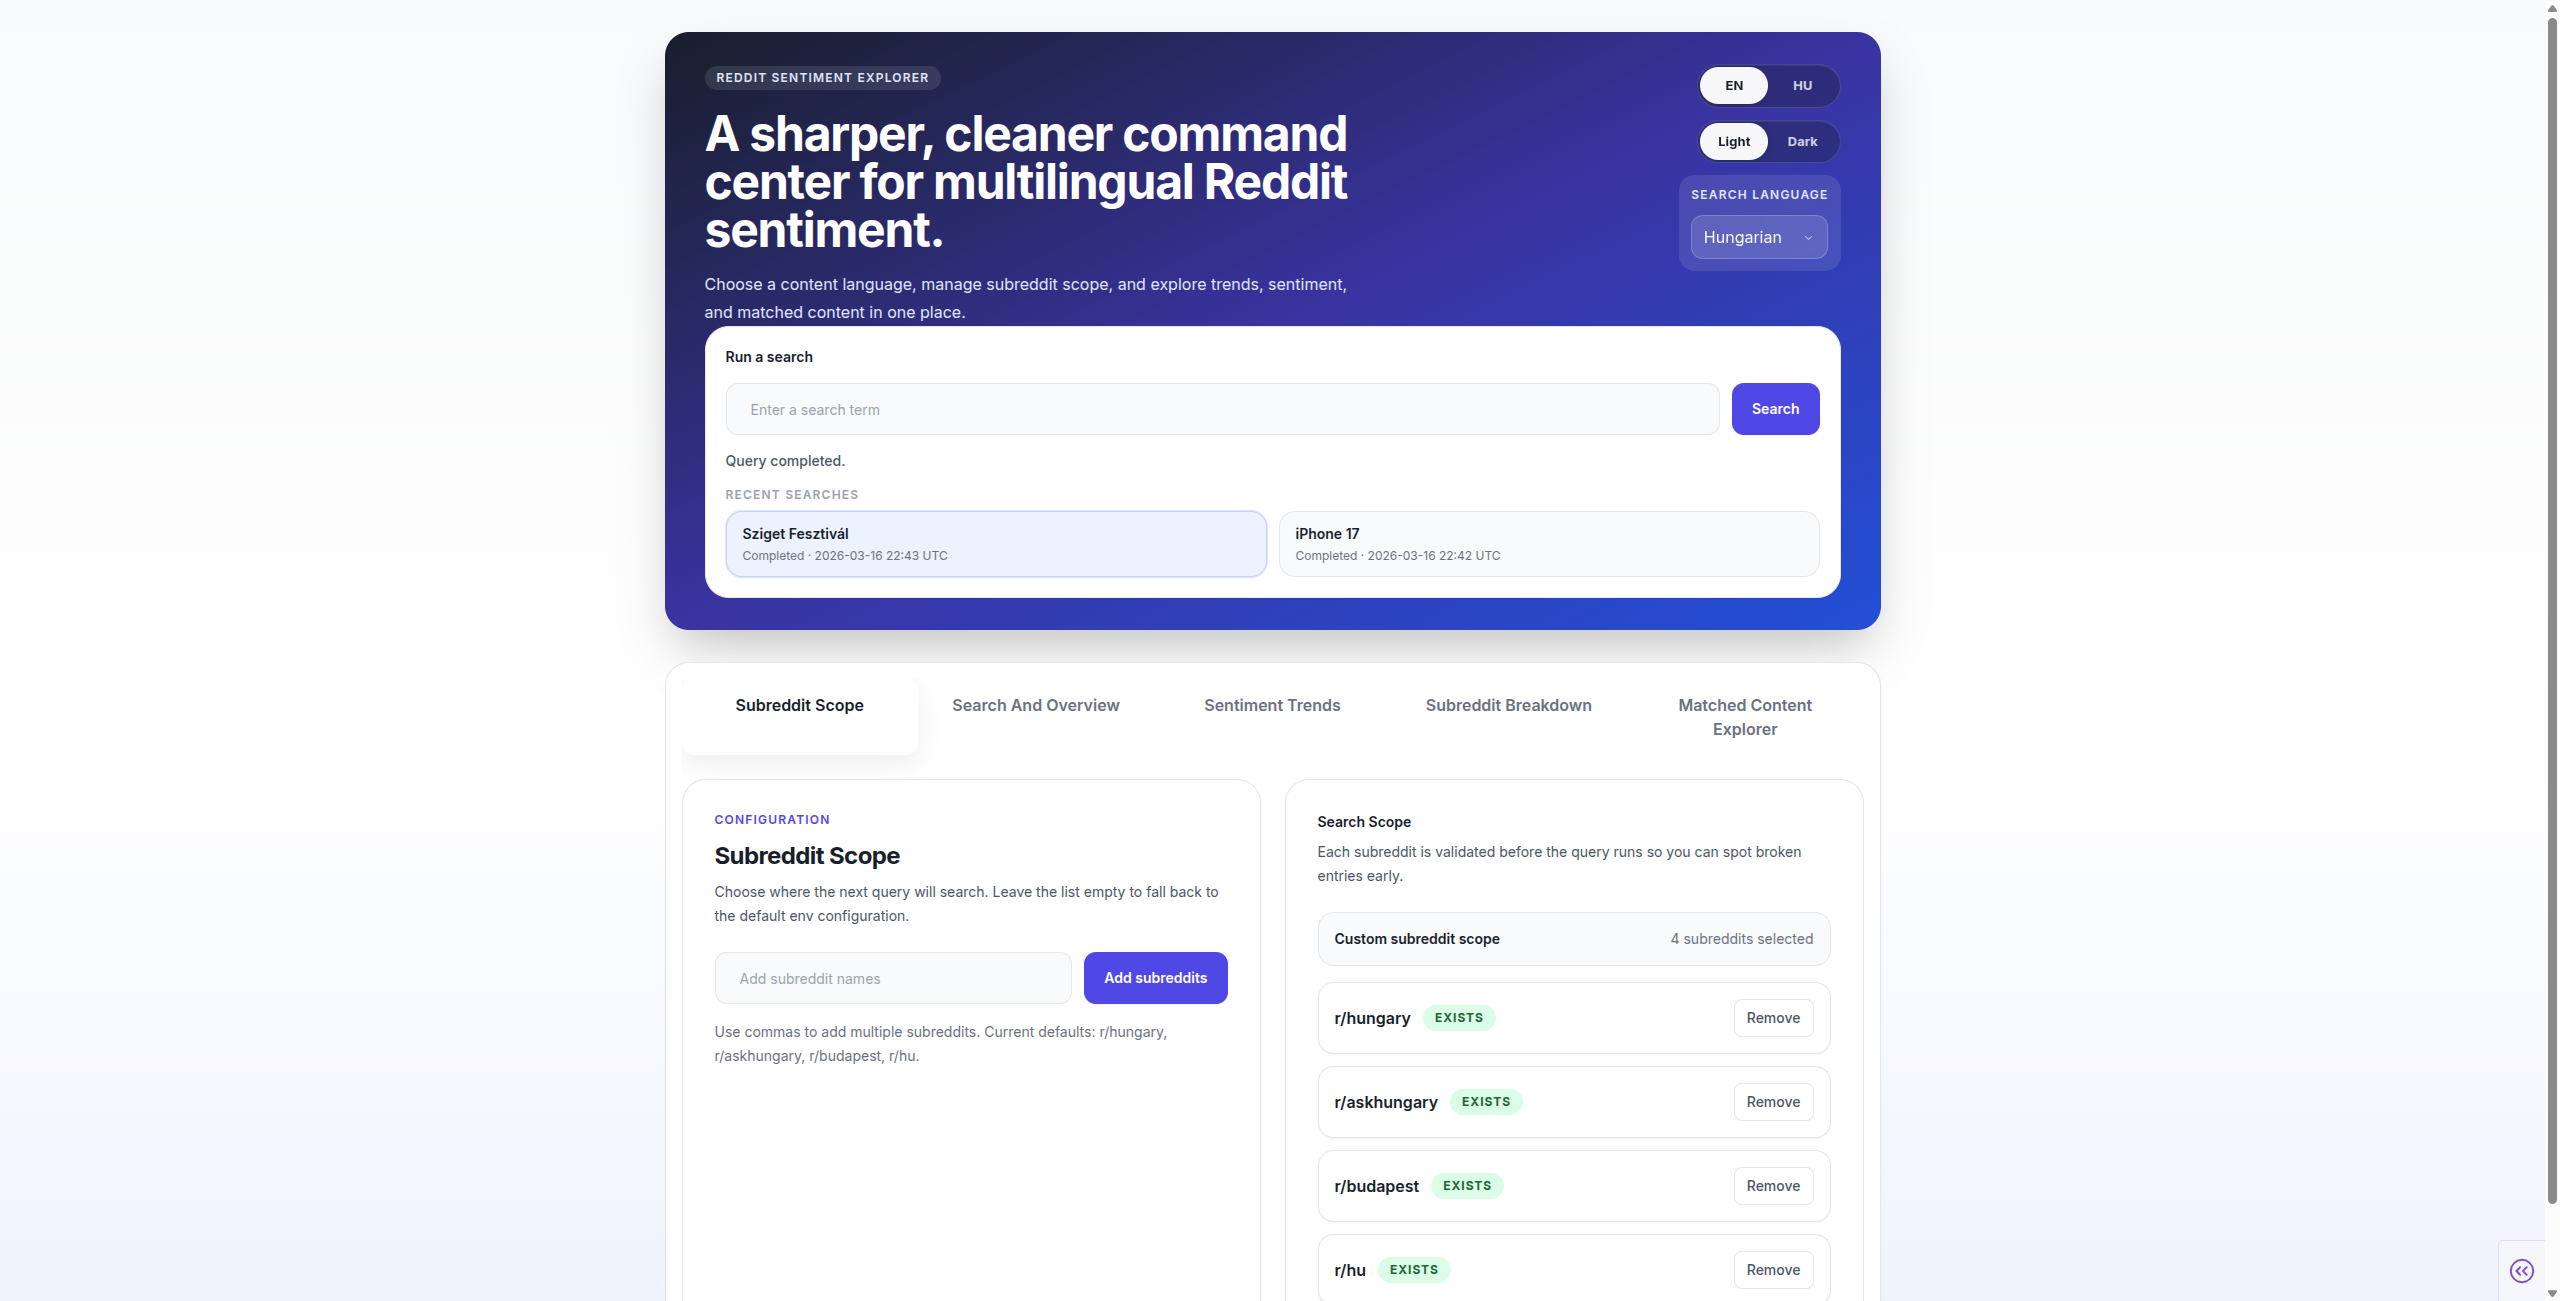
\includegraphics[width=\textwidth]{figures/dashboard-hero.png}
    \caption{Dashboard landing page with search interface and subreddit scope management.}
    \label{fig:appendix_dashboard}
\end{figure}

\begin{figure}[H]
    \centering
    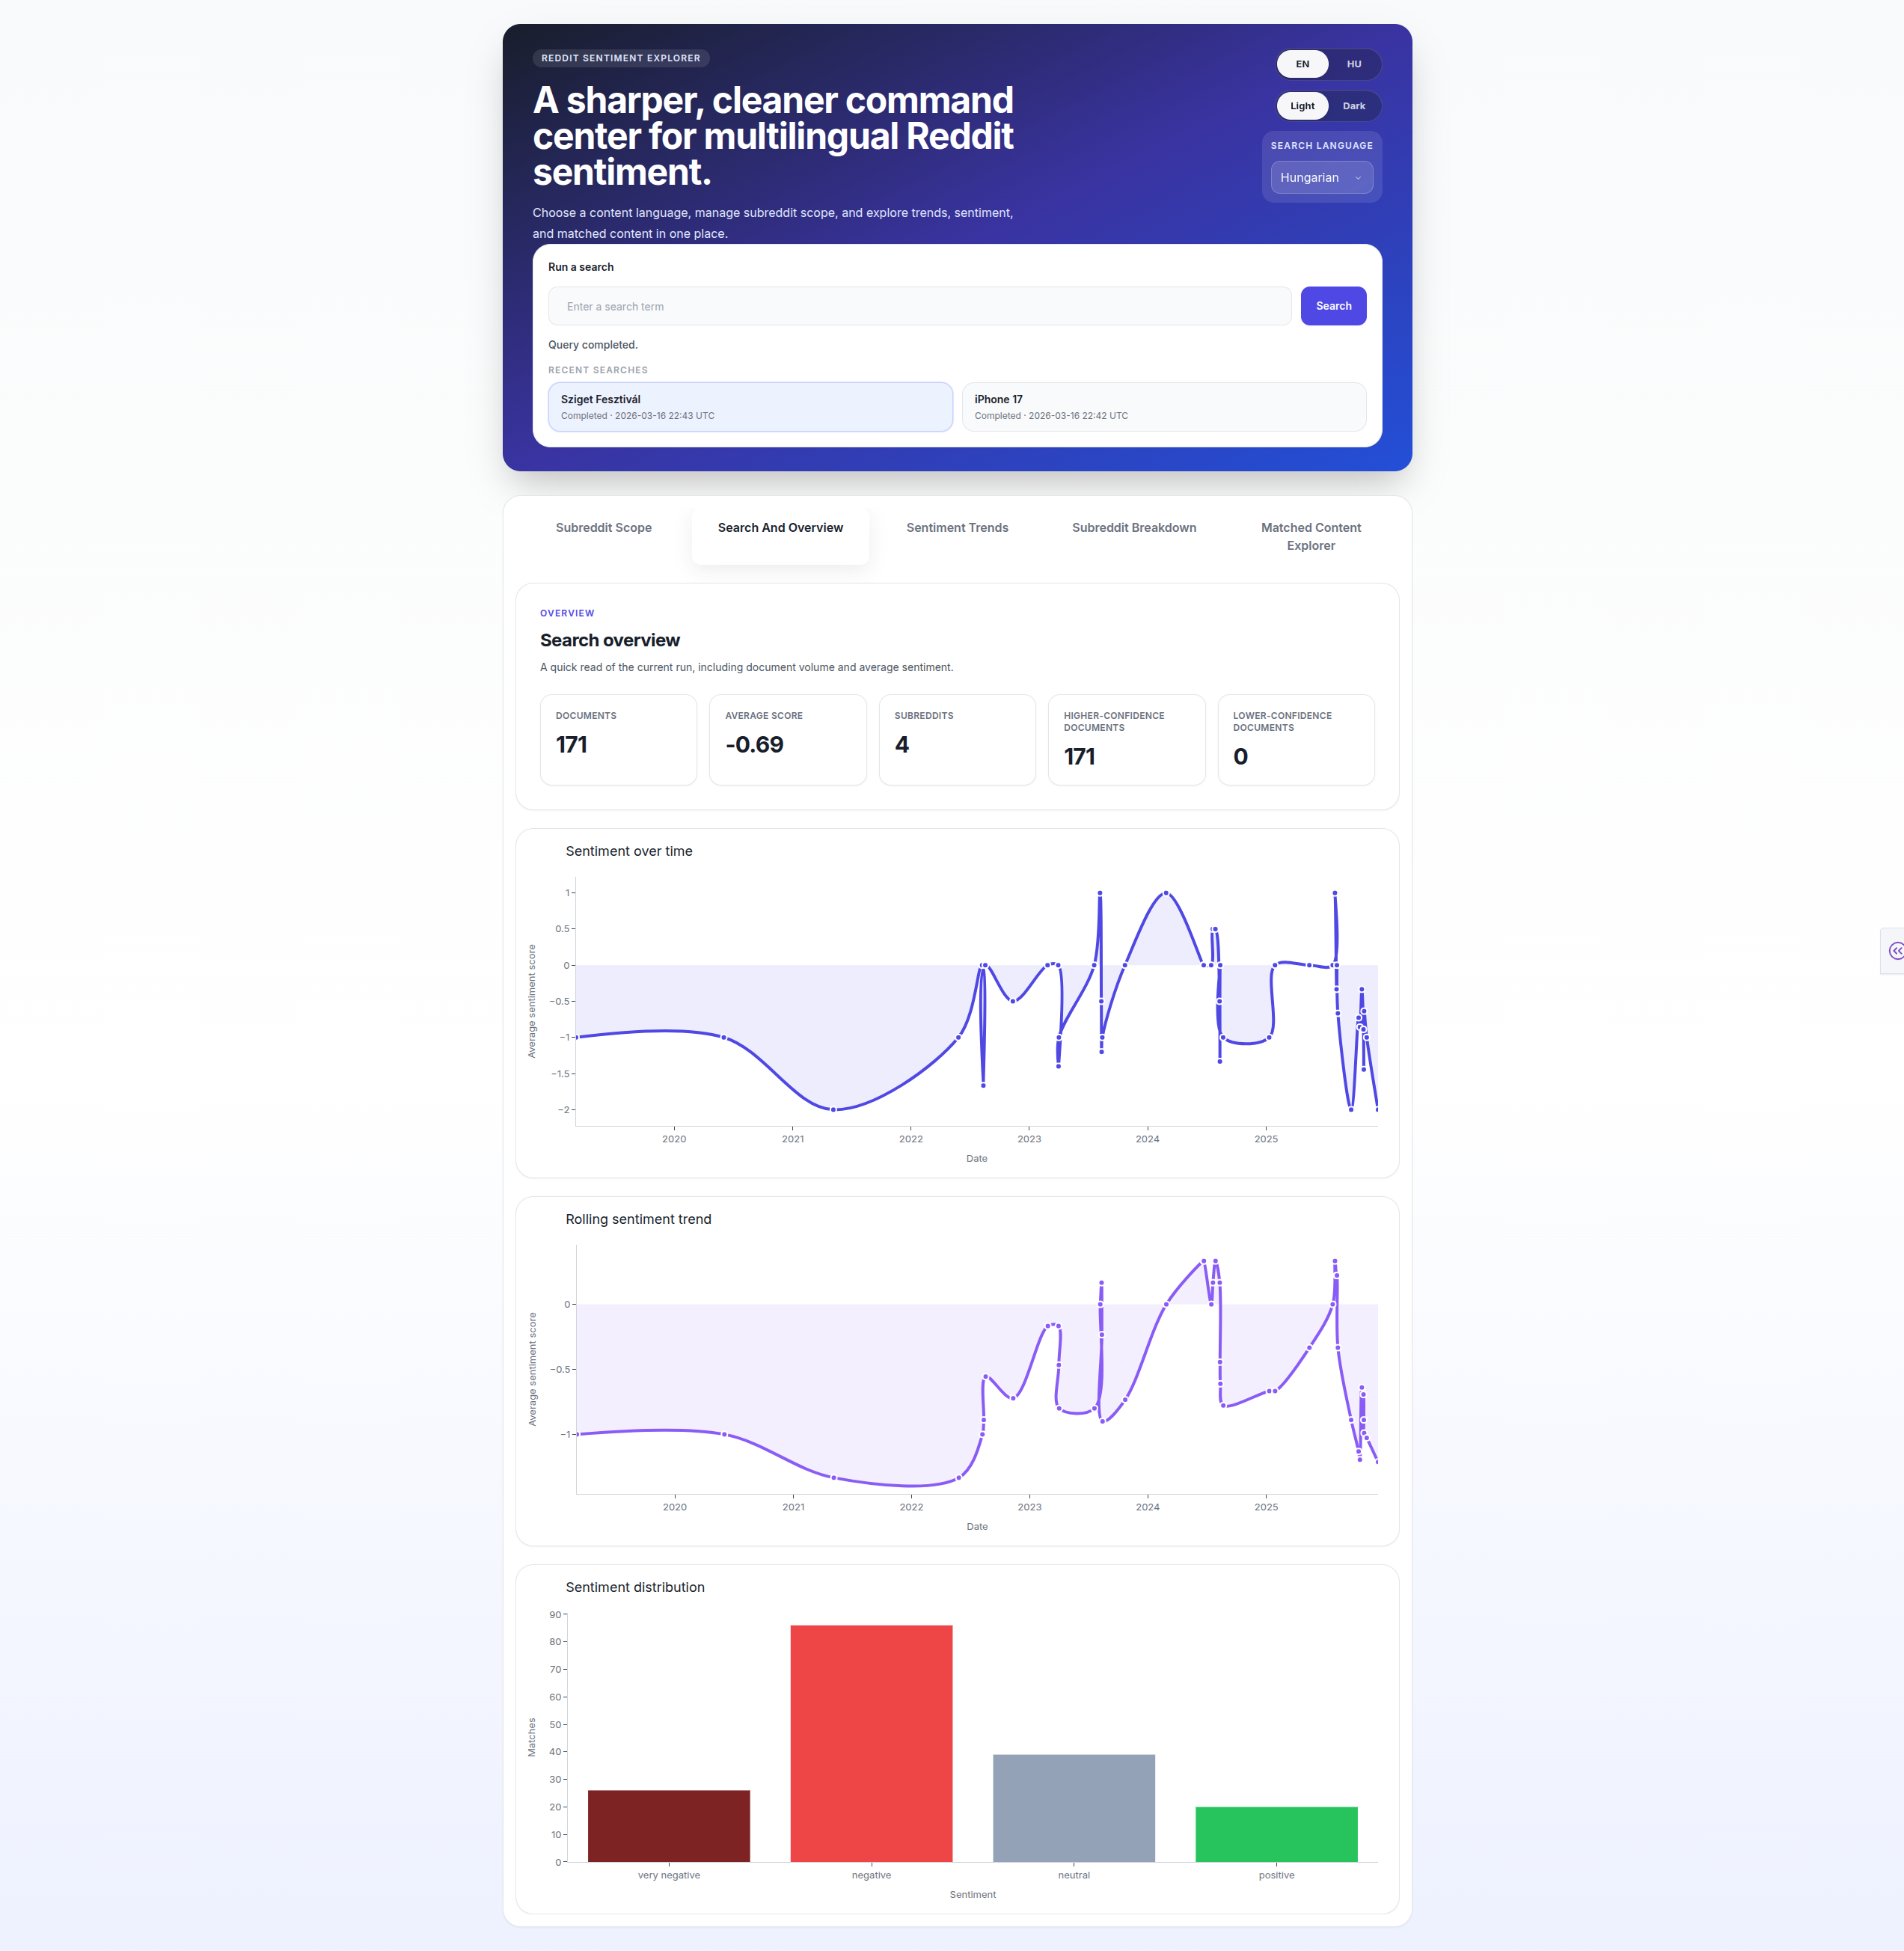
\includegraphics[width=\textwidth]{figures/search-overview.png}
    \caption{Search And Overview tab with overview metrics, sentiment timeline, rolling sentiment trend, and sentiment distribution charts.}
    \label{fig:appendix_overview}
\end{figure}

\begin{figure}[H]
    \centering
    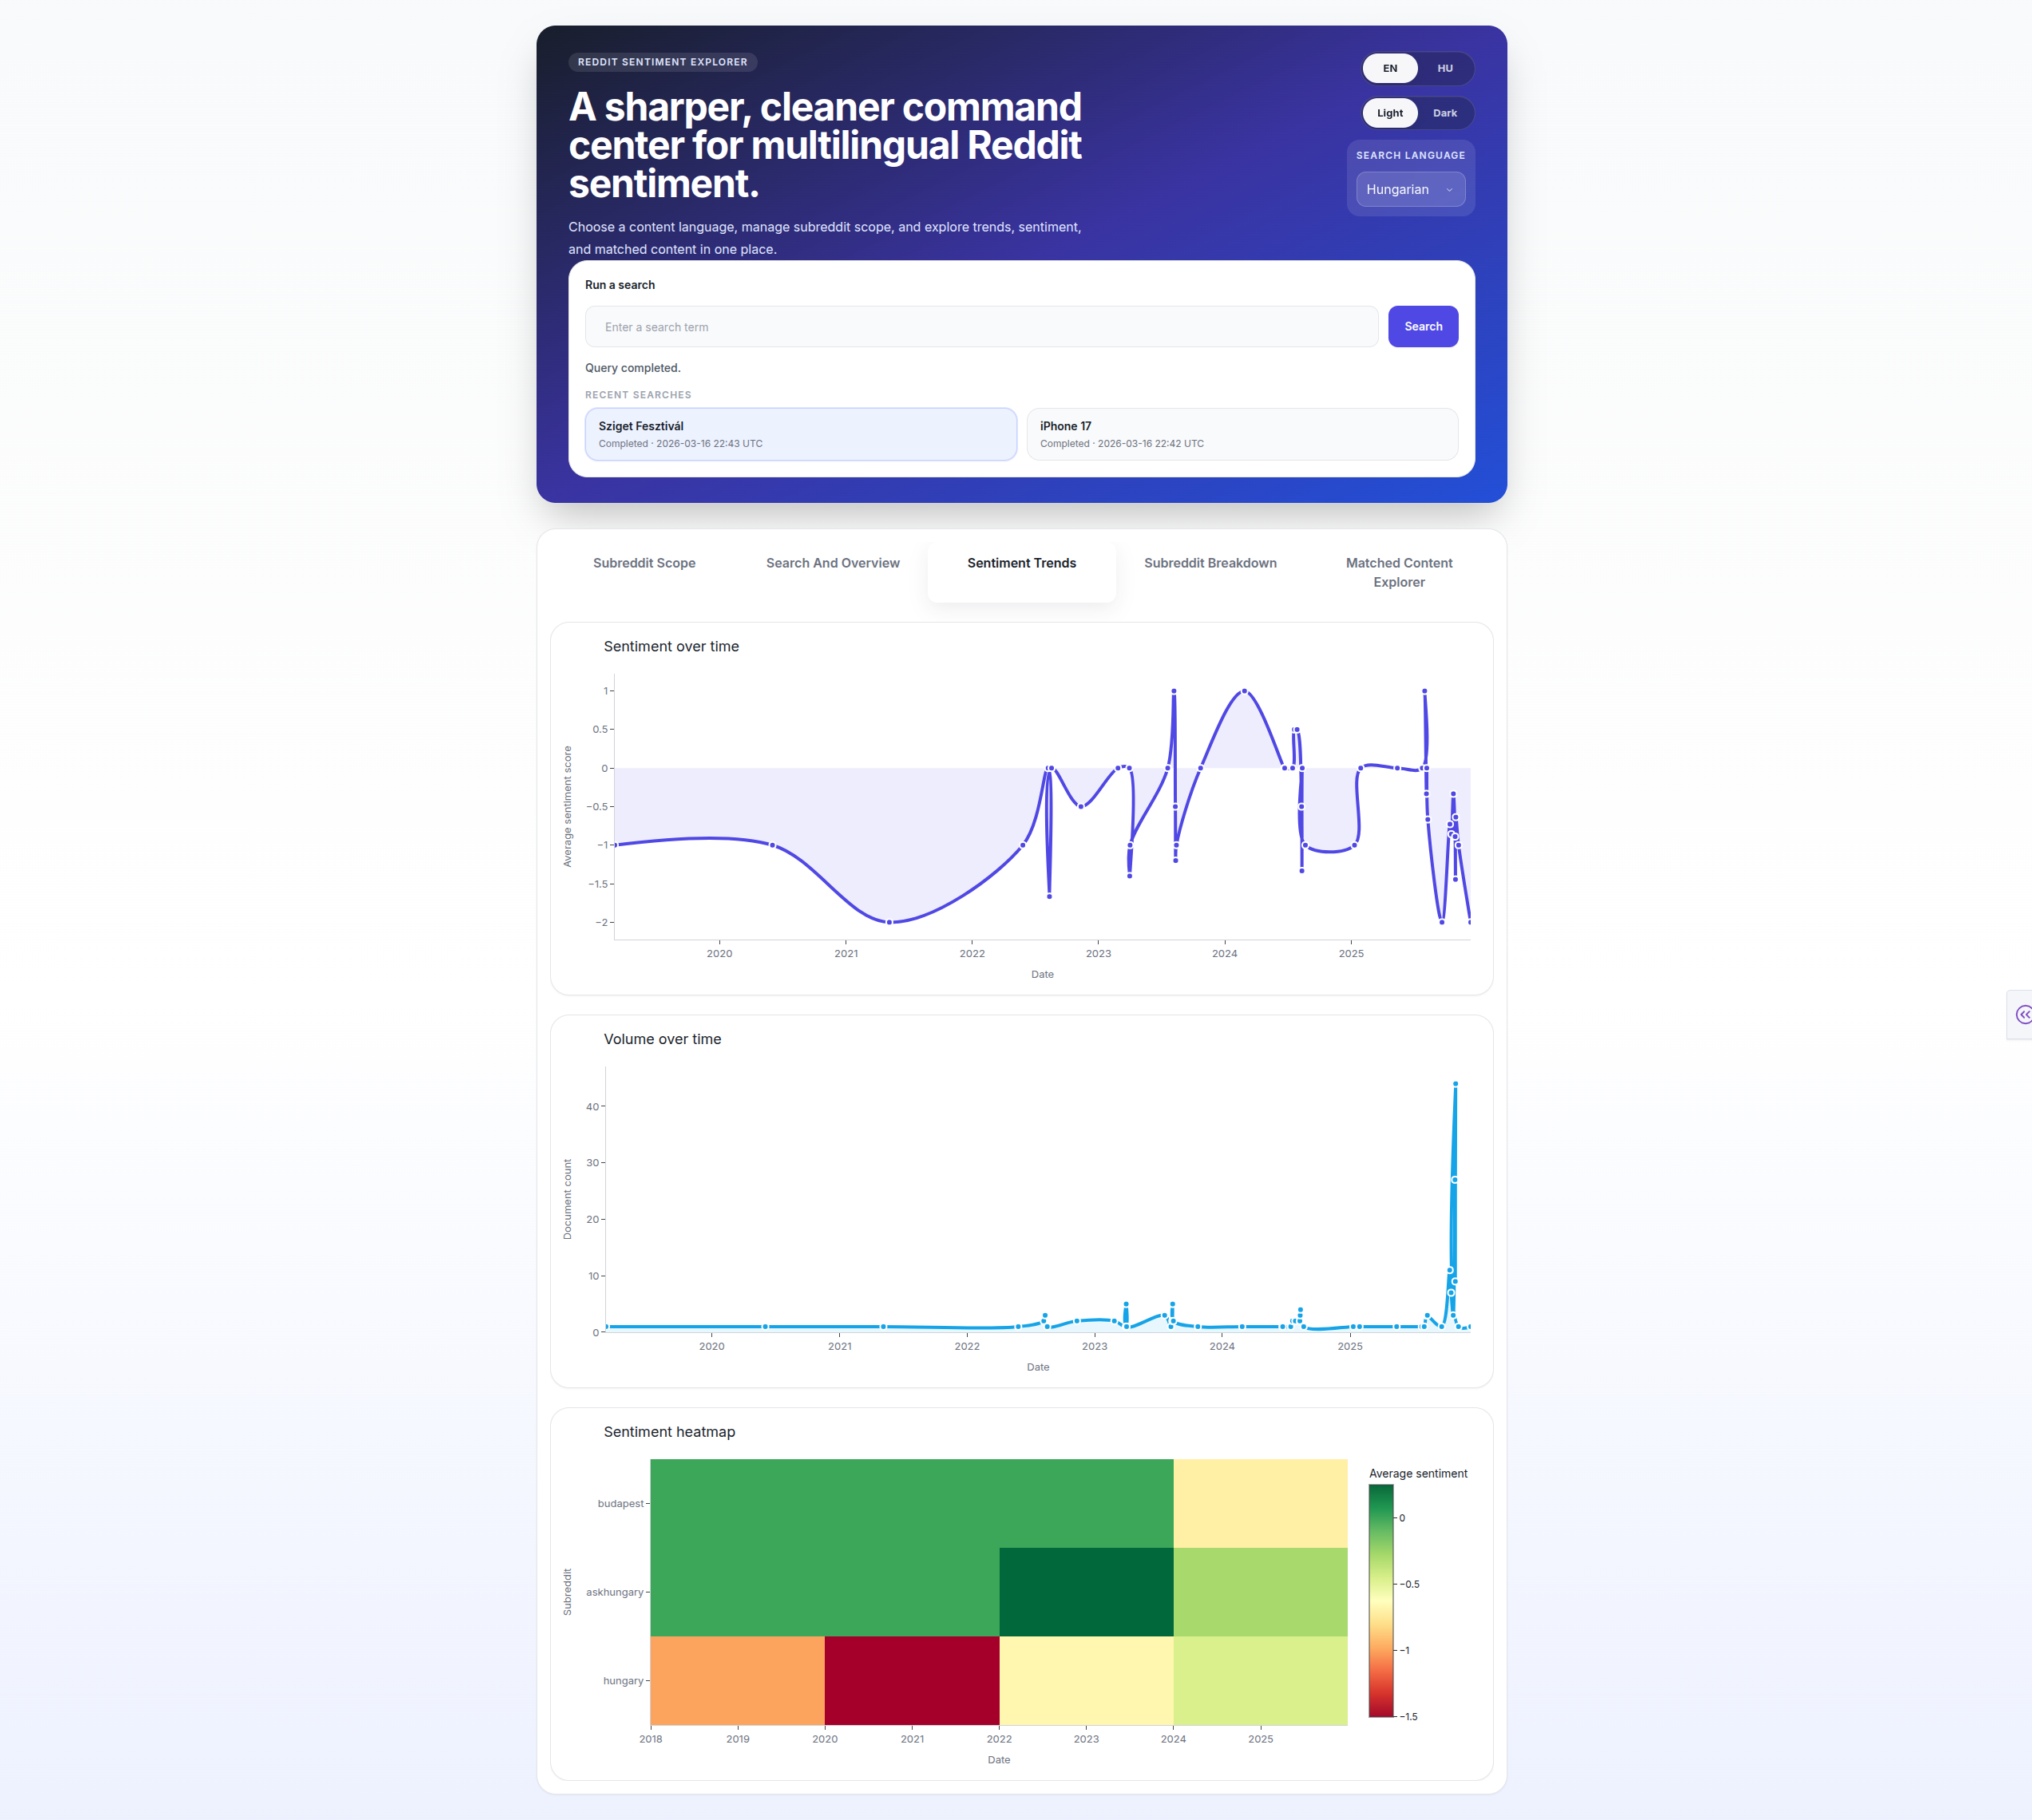
\includegraphics[width=\textwidth]{figures/sentiment-trends.png}
    \caption{Sentiment Trends tab with sentiment timeline, volume timeline, and sentiment heatmap.}
    \label{fig:appendix_trends}
\end{figure}

\begin{figure}[H]
    \centering
    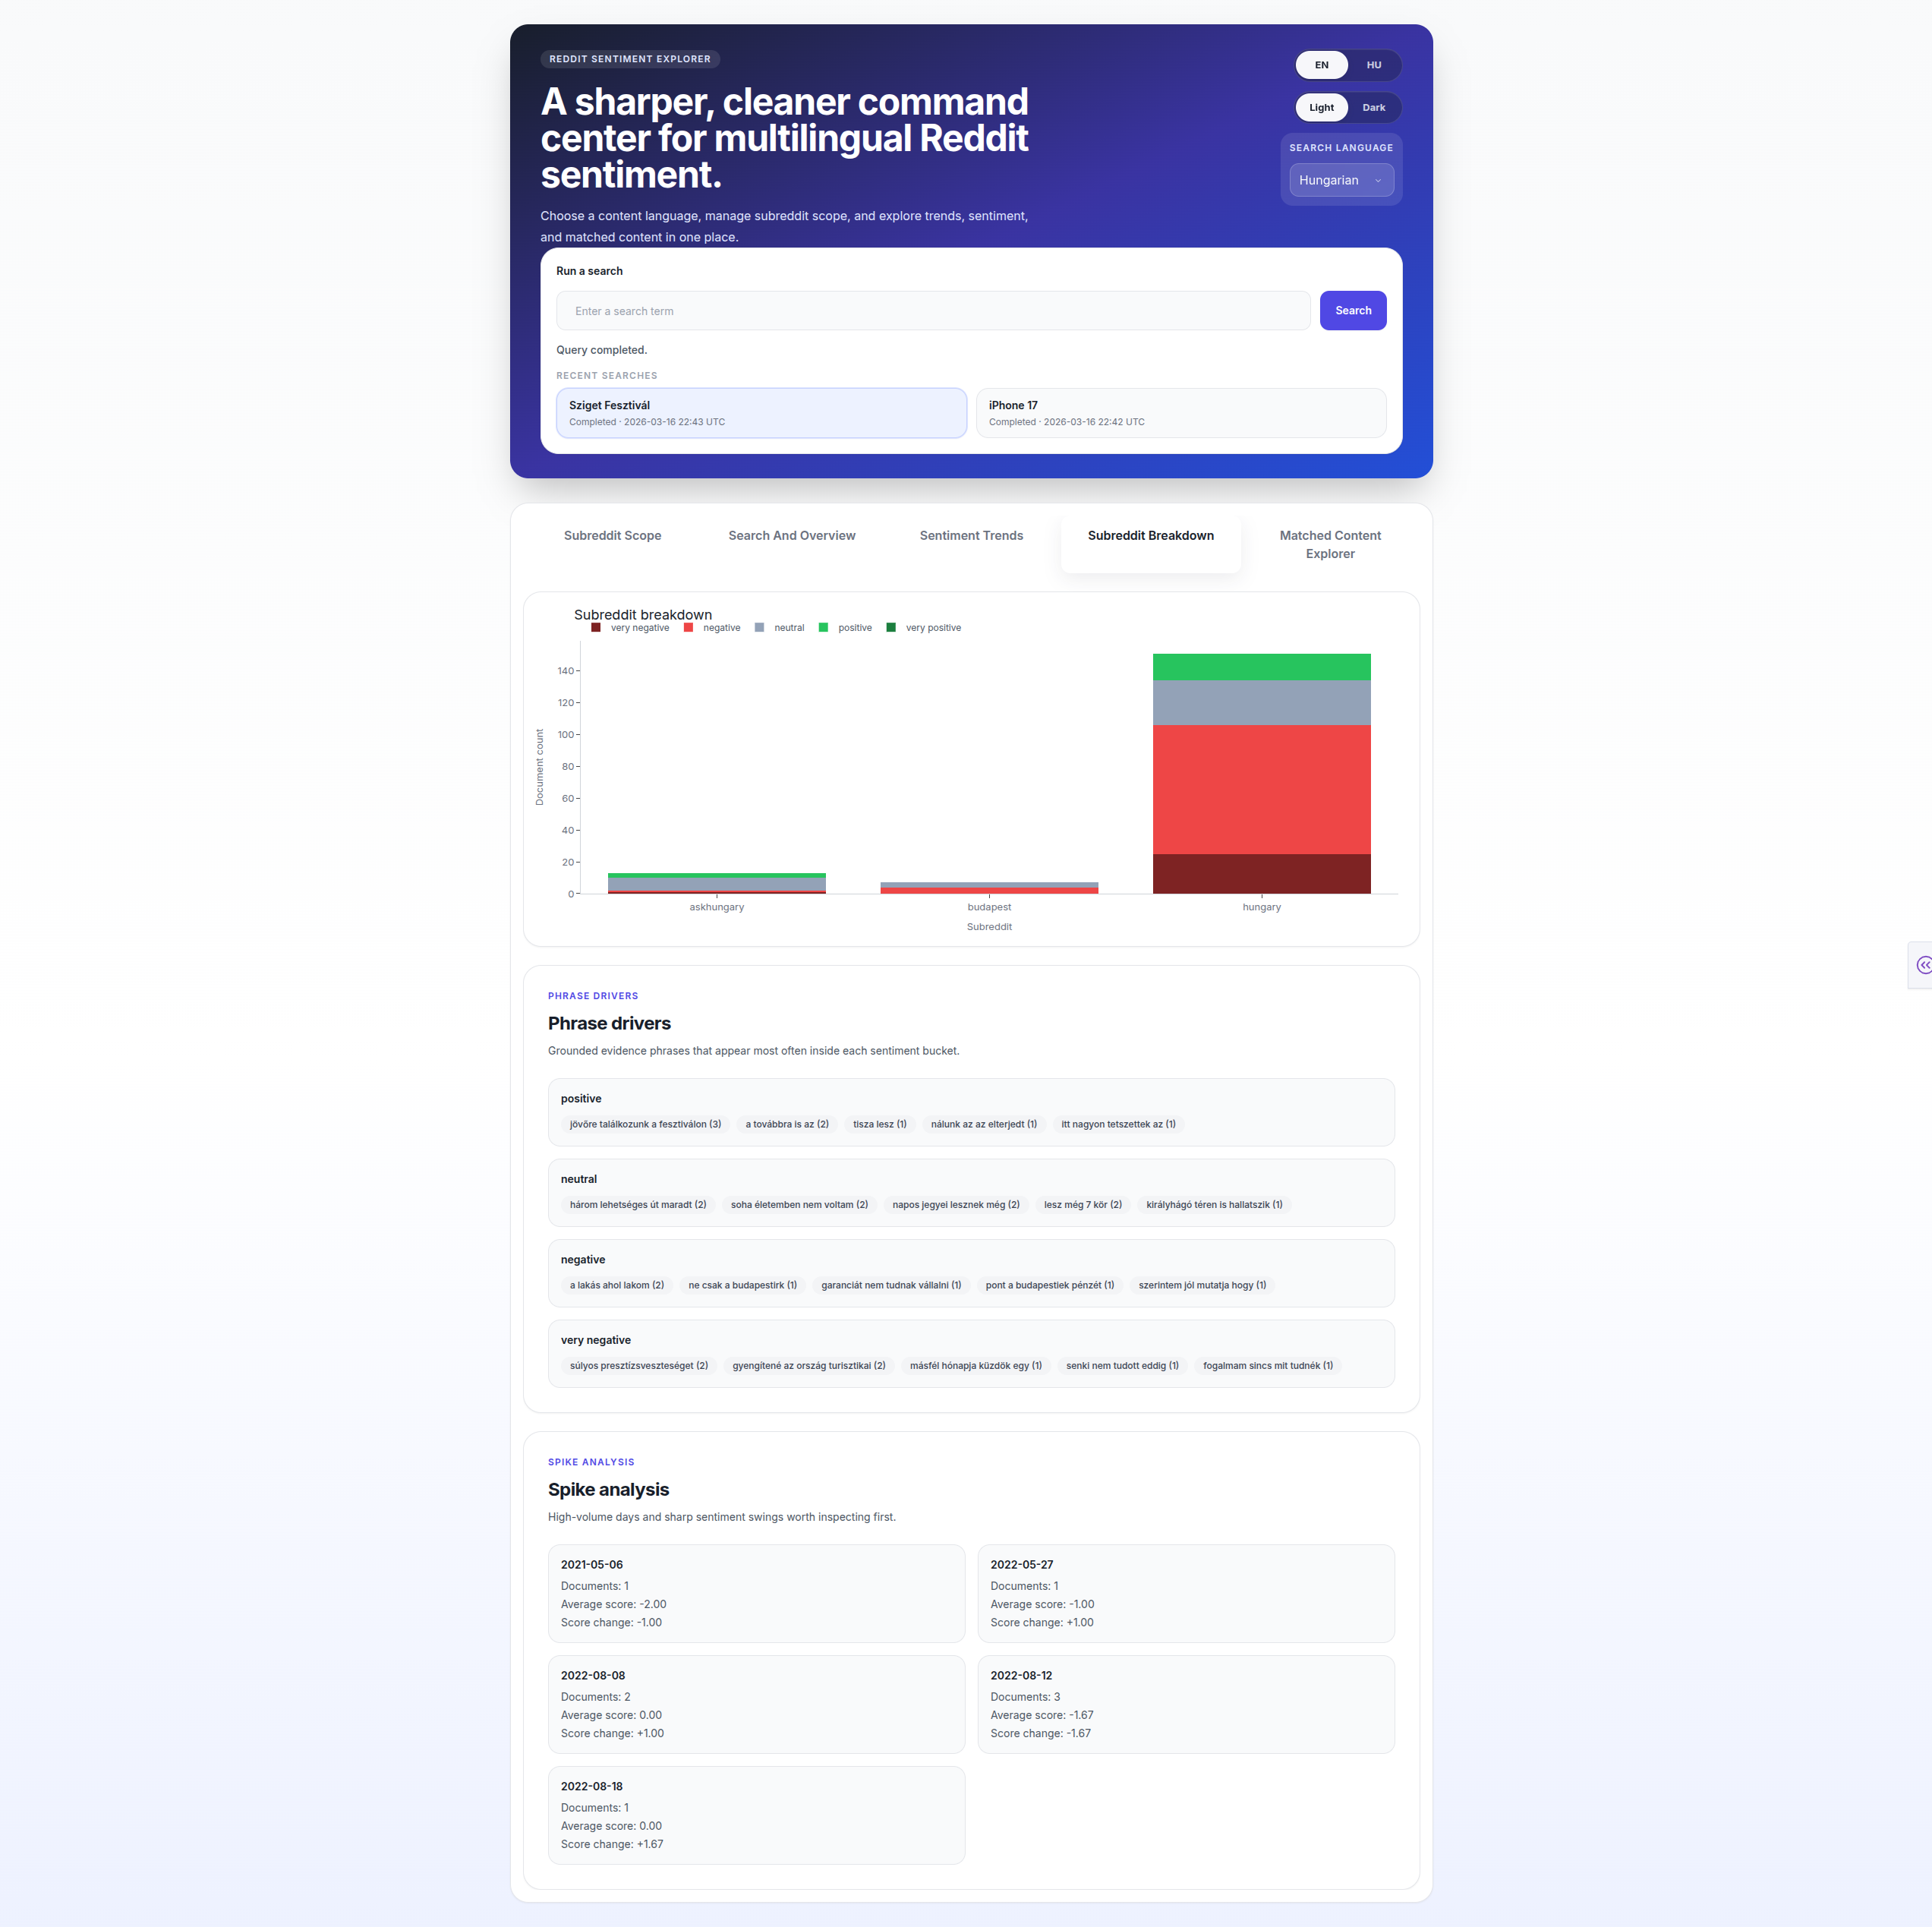
\includegraphics[width=\textwidth]{figures/subreddit-breakdown.png}
    \caption{Subreddit Breakdown tab with per-subreddit chart, phrase drivers, and spike analysis.}
    \label{fig:appendix_breakdown}
\end{figure}

\begin{figure}[H]
    \centering
    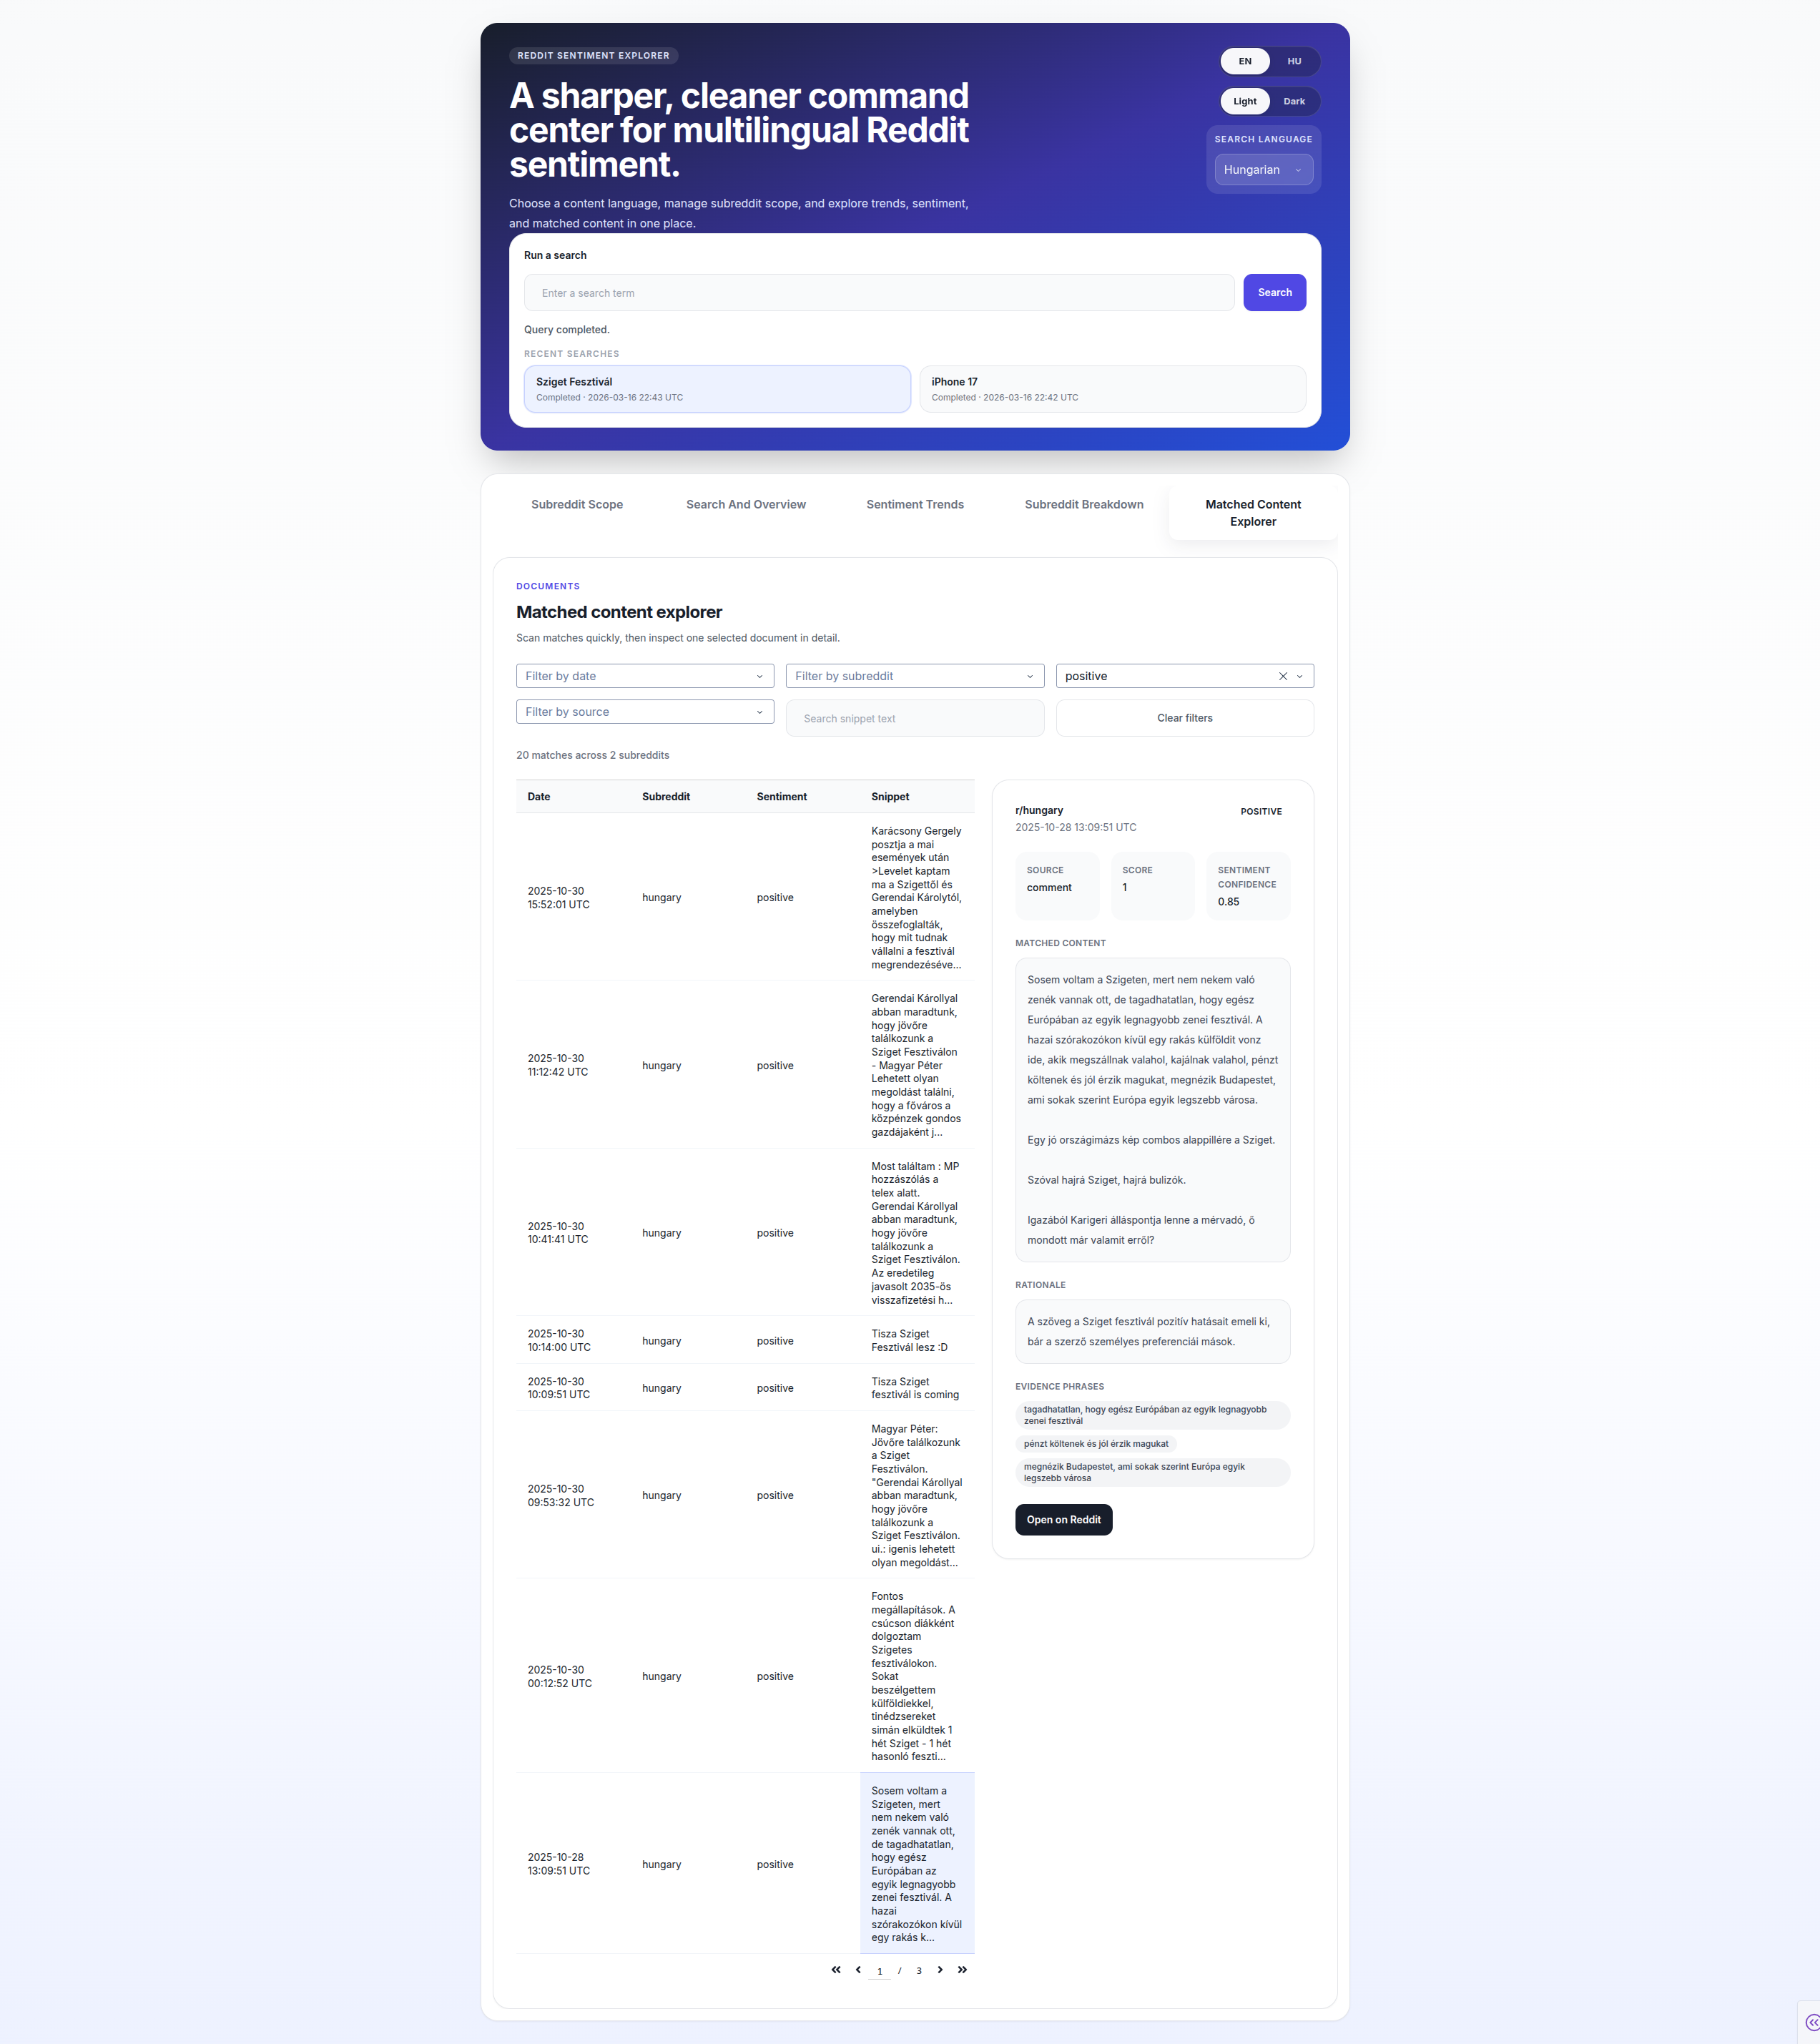
\includegraphics[width=\textwidth]{figures/matched-content.png}
    \caption{Matched Content Explorer with document details, sentiment rationale, and evidence phrases.}
    \label{fig:appendix_matched}
\end{figure}


\end{document}
